\documentclass[a4paper]{article}

%% Language and font encodings
\usepackage[english]{babel}
\usepackage[utf8x]{inputenc}
\usepackage[T1]{fontenc}

%% Sets page size and margins
\usepackage[a4paper,top=3cm,bottom=2cm,left=3cm,right=3cm,marginparwidth=1.75cm]{geometry}

%% Useful packages
\usepackage{filecontents}
\usepackage{amsmath}
\usepackage{algorithm}
\usepackage[title]{appendix}
\usepackage{algorithmic}
\usepackage{listings}
\usepackage{graphicx}
\graphicspath{{images/}}
\usepackage{float}
\usepackage{listings}
\usepackage{amssymb}
\usepackage{latexsym}
\usepackage{amsfonts}
\usepackage{epsfig}
\usepackage{mathrsfs}
\usepackage{mathtools}
\usepackage{enumitem}
\usepackage{bashful}
\usepackage{array}
\usepackage{subfig}
\usepackage{url}
\usepackage[colorinlistoftodos]{todonotes}
\usepackage[colorlinks=true, allcolors=blue]{hyperref}
\usepackage{titlesec}
\usepackage{enumitem}
\usepackage[title]{appendix}
\setlength{\parindent}{0pt}
\setlength{\parskip}{1.5em}

\setcounter{secnumdepth}{4}

\titleformat{\paragraph}
{\normalfont\normalsize\bfseries}{\theparagraph}{1em}{}
\titlespacing*{\paragraph}
{0pt}{3.25ex plus 1ex minus .2ex}{1.5ex plus .2ex}
\begin{document}
\title{Using NLP and Geopolitical Events Presented in the Global Database for Events, Language, and Tone to Perform Predictive Modelling on Stock Market Data}
\author{Jalaj Khandelwal\\Student ID: 160001602}
\date{}
%\setcounter{secnumdepth}{-2}
 \thispagestyle{empty}
	
	\begin{titlepage}
		\vspace{\fill}
		\maketitle
		 \thispagestyle{empty}
		\begin{figure}[H]
			\centering
			
\includegraphics[width=0.4\textwidth]{Images/SchoolLogo.png}
		\end{figure}
		\begin{center}
			\Large\textbf{University of St Andrews}\\
			\vspace{1cm}
			\Large\textbf{School of Mathematics and Statistics}
		\end{center}
		
		\vspace{\fill}
		\Large%\textbf{Details}
		\begin{itemize}
			\renewcommand\labelitemi{--}
			\item[] \textbf{Supervisor}: Dr Carl Donovan  
			\item[] \textbf{Module}: MT5099 Masters Dissertation in Partial Fulfillment of the MSc.\ in Data Intensive Analysis
			\item[] \textbf{Date}: \today
		\end{itemize}
		\vspace{\fill}
	\end{titlepage}



%\setcounter{secnumdepth}{-1}
\section*{Declaration}
\addcontentsline{toc}{section}{Declaration}
I hereby certify that this dissertation, which is approximately 14,500 words in length, has been composed by me, that it is the record of work carried out by me and that it has not been submitted in any previous application for a degree. This project was conducted by me at University of St Andrews from June 2020 to August 2020 towards fulfilment of the requirements of the University of St Andrews for the degree of MSc. in Data Intensive Analysis under the supervision of Dr Carl Donovan.

17th August 2020

Jalaj Khandelwal
\section*{Abstract}
\addcontentsline{toc}{section}{Abstract}
This Masters Dissertation was focused on trying to use geopolitical events to predict changes in the stock market. This aim was to first use the Global Database for Language and Tone (GDELT) to build topic models, which organise the geopolitical news into topics which could be used as a filter for the daily news cycle. Then, using the Tone and Geopolitical conflict scores provided by GDELT, models would be made made to predict changes in the stock market. There were two main topic modelling approaches, firstly using Latent Dirichlet Allocation, and secondly using K-Means clustering with TF-IDF. Both of these approaches either were incapable, or struggled to filter unseen news effectively, which means that they would not be effective in picking up new topics. However, many different stock predictive models were tried, and it was found that the accuracy of models using information provided by GDELT was higher in predicting binary stock shift, compared to a model which just only used the previous day's stock shift as a predictor. The best of the models also were able to demonstrate adding value to a simple portfolio, which suggests that using GDELT is a viable metric by which to predict the stock market. 
\section*{Impact of COVID-19}
The impacts of COVID-19 was minimal on this dissertation. The only issue was the amount of data used being restricted due to the machine constraints. Without Covid-19 data covering a longer time period from GDELT would have been used.
\newpage
\tableofcontents
\listoftables
\newpage
\listoffigures


\section{Introduction}
This is my dissertation 

\section{Existing Work}

There exist many approaches, and many different models to aim to predict stock prices. These approaches use many different sources of data, and many different modelling styles to predict stock prices. It is common to use sentiment analysis to predict stock prices for example. However, there remains limited prior work in modelling stock prices using calculated Geopolitical risk, though there are limited approaches to calculating geopolitical risk on its own.

\subsection{Geopolitical risk}
The majority of approaches in modelling Geopolitical risk work on using news information along with manually defined terms of geopolitical risk. One of the most recent approaches was done by Dario Caldara and Matteo Iacoviello, where they created a Geopolitical risk index from a series of news articles \cite{caldara2018measuring}. 

This risk index was calculated by manually creating search terms which define geopolitical risk in several categories, and then over time calculate the percentage of articles of selected number of news media in which the search terms appear. This is then used to model against the stock prices.

There are other risk measures present, Black Rock also have a publicly viewable index called the BlackRock Geopolitical Risk Indicator (BGRI) \footnote{https://www.blackrock.com/corporate/insights/blackrock-investment-institute/interactive-charts/geopolitical-risk-dashboard}, which works in a similar fashion where key words are selected which define geopolitical risk, followed by an application of a sentiment score from a list of predefined words, and then those two scores are combined to make the BGRI total score. Furthermore, there are also many other organisations which almost certainly will model Geopolitical Indices, such as Reuters, but will not disclose the exact modelling for proprietary purposes.

One of the major differences between the existing approaches in modelling geopolitical risk and the approach this dissertation attempted to use the cooperation conflict scale provided in GDELT. The main differences are that GDELT does not restrict which news media are used for reference, instead using more than any other . Furthermore, this approach attempts to use topic modelling to filter the news, as opposed to using manually defined search terms, in an attempt to make the prediction process more automated. 

\subsection{Modelling Stock Prices}
There is a large vested interest for people to aim to model the stock market effectively, as any investor with extra knowledge about where the market will go will be able to take a position most beneficial to them. Thus, there are a large number of models which exist and are used which aim to predict the changes in the markets. 

The efficient markets hypothesis claims that markets are rational and act upon indicators which can be predicted. This means that Geopolitical events, and by extension an index of risk should have a measurable effect on stock prices, in that, if the risk increases if an bad event occurs or a negative piece of news is published, it would be assumed that stock prices would decrease as people would be more likely to sell which would cause the decrease in the price, and vice versa.

As stock market modelling has existed for many years there have been many esoteric factors used to model and predict stock prices aside from the news, such as the weather on Wall Street \cite{saunders1993stock}. For most of the non quantitative data, sentiment analysis is commonly used to help predict stock prices, where natural language processing is used to gain a measure of tone in data being used, and from that, the changes in the price is modelled. This is similar to the average tone measured by the GDELT. However, there is limited prior work using information at the scale of which GDELT provides. However, a number of studies shows that large amounts of data on social medias such as Facebook and Twitter can be useful for forecasting economic indicators such as the stock market \cite{bollen2011twitter} \cite{arias2014forecasting}. 

With regards to the models themselves, there are many different machine learning and statistical models used. The aforementioned geopolitical risk index worked on by modelling the stock price against the risk index using Vector Autoregressive Regression models. 

One of the simplest approaches to stock price modelling is to perform autoregressive modelling on purely the time series data for stock prices. In this approach, the only thing which is used to predict the prices are the past values of the stock. One common approach is to use an ARIMA model \cite{ariyo2014stock}, which is an autoregressive integrated moving average, which expresses Y as a linear combination of p past values multiplied by the weights. This aims to extract information from the previous p days to gain a balanced view of where the stock prices are likely to go on a day by day basis (or the time period being modelled).  

When predicting stock prices from dependant variables as opposed to just from the previous meetings, many different machine learning algorithms are used. Aside from classical regression algorithms, these include SVMs \cite{cao2003support}, Random Forests \cite{khaidem2016predicting}, and Neural Networks \cite{egeli2003stock}, along with more Bayesian approaches such as Naive Bayes \cite{khedr2017predicting}. These are generally regression predictors which aim to predict the stock prices themselves. However, there are algorithms which try and predict stock shift as opposed to prices, i.e. whether the market and prices have gone up or down \cite{nguyen2015sentiment}.  

More broadly, there is another concern with modelling on the stock market. When predicting any stock market, one of the major issues which arises is that in the long term the stock market always grows, for the S and P for example there is an annualised growth of on average 9.5\% (Macrotrends. S\&P 500 Historical Annual Returns) without the affect of inflation factored in. Thus any investor investing over a sufficiently long period of time will nearly always make money. The aim then, is to build models which would give better results than the normal stock market rise, and thus any strategy or predictions by any model would have to prove and provide better returns than just investing in the long term growth of the stock market.

A mixture of these algorithms were used alongside the GDELT algorithm to try and predict stock shift. 


\section{GDELT}
\label{gdelt}

The Global Database for Events Language and Tone was the basis for this dissertation. This is a database which stores a record of every broadcast, print, and web news published since 1979, in over 100 languages from all parts of the world. 

The records are stored across multiple database tables accessible either directly, or through SQL in Google Big Query. The main table which was the source of the data in this dissertation was the Events table. This table maintains the record of all events, along with cursory information about each event, such as which countries it happened in or between, the dates, and the URLs of the first news article this appeared in. The events table contains over a quarter of a billion georeferenced records each referring to an event which occurred since the 1st of January 1979. 

For each event, there are three variables of note for this dissertation, the source URL, the Average Tone and the Goldstein Scale. The source URLs were the URLs of the first headline which covered the event. The topic models were built on these headlines of the articles extracted from the source URLs, where present. The Average Tone is a measure of the sentiment of all the news media which describes the specific event. It is on a scale of -100 (Extremely Negative) to +100 (Extremely Positive). The most common values observed are usually between -10 and 10, and 0 indicated a neutral tone. 

The Goldstein Scale is the main metric by which geopolitical modelling occurs, and was initially defined as the Conflict-Cooperation Scale for Work Environment Impact Scale (WEIS) events data \cite{goldstein1992conflict}. This is a scale between -10 and +10 which captures the potential impact an event will have on the stability of the entity in question (usually a country), with -10 being the worst impact an event can have and +10 being the most positive impact an event can have. It should be noted that these numbers are predefined and do not take into consideration the extent to which an event occurs, for example event type 071, Extending economic aid; give, buy, sell, or borrow, is given a score of +7.4, regardless of whether it is £1 of aid given or £1 million. 

GDELT has been used for stock predictions in the past \cite{memari2017predicting} \cite{alamro2019predicting}, however, it is used much more commonly used for predicting and analysing geopolitical events themselves \cite{qiao2017predicting} \cite{yonamine2013predicting}. 
\section{Topic Modelling}
\label{topic}
Topic Modelling is an unsupervised machine learning and statistical modelling approach which aims to discover the abstract `topics` in a collection of documents, referred to as the corpus. This can be used to find hidden semantic structures in a document. This works by looking at how often words appear in the corpus and trying to create topics made of words which are related to each other. For example an article about dogs would be more likely to have words such as `dog` and `bone`, and thus the topic model would most likely group those two words together into a topic. 

There are many approaches to topic modelling, one of the foremost examples is Latent Dirichlet Allocation \cite{blei2003latent}, which aims to reverse-engineer the topics by assuming the text was created from K topics and all words directly relate to one of the K topics. There are other forms of clustering algorithm which can be applied to words, such as the K-Means clustering algorithm. 

\subsection{Latent Dirichlet Allocation}
Latent Dirichlet Allocation (LDA) is an unsupervised learning model which aims to collate words into K topics. When performing LDA, the text to be analysed is split into a series of documents, each composed of a bag of words where the order of the words does not matter. Most of the time, this will require pre-processing to remove words which do not contribute to the topics present in the work such as `the`, `is`,  and `a`. 

\noindent This algorithm assumes that the documents was made by first picking K topics, and any words present in the document belong to one of those K topics. The algorithm aims to reverse-engineer this process.
% START HERE 

Initially if the corpus is composed of a set of documents, D, the algorithm would first perform tokenisation so that each individual word is treated as a unique identity. Then each of the tokens for each of the documents would be parsed to remove the stop words. At this point each document is a list of tokens representing words which are not stop words. From this a document term matrix is created. This matrix has the dimensions $m$ x $v$, where M is the number of documents present in the corpus. V is the number of unique words present across all of the documents, or the vocabulary. This document term matrix records the term frequency of all of the words in the vocabulary for all of the documents present.

\begin{figure}[H]
	\centering
	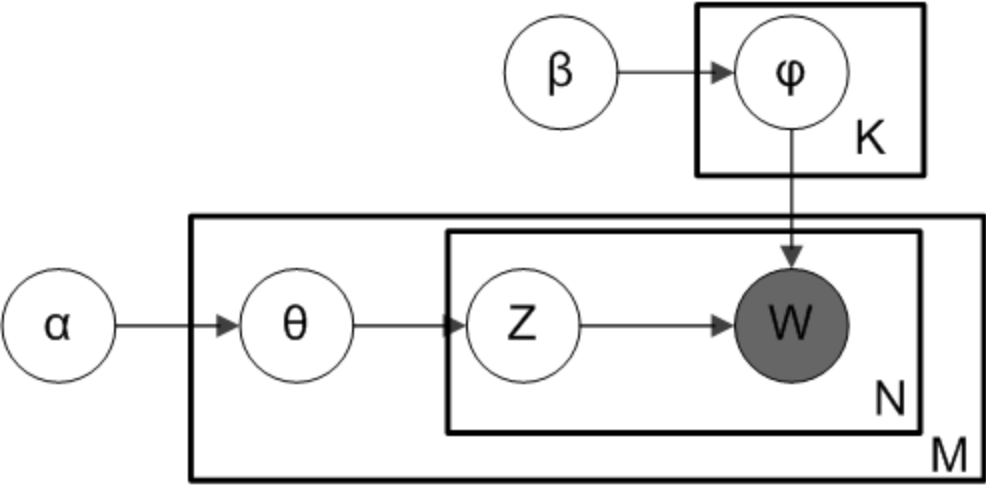
\includegraphics[width=0.6\textwidth]{images/LDA.png}
	\caption{A Graphical Plate representation of (smoothed) LDA (image from \cite{LDA})}
	\label{fig:ldafigure}
\end{figure}

The reverse-engineering process is shown graphically in Figure \ref{fig:ldafigure}. M denotes the number of documents, N refers to an individual document, and W refers to a single word, and is the only observable variable in the system. The algorithm assumes several matrices. \boldmath{$\varphi$} is defined as the word distribution across topics. In practice this is a matrix where \boldmath{$\varphi_{k}$} is the probability distribution across the V for topic K, such that \boldmath{$\varphi_{j, k}$} represents the probability that the \unboldmath{$j^{th}$} word in the vocabulary belongs in topic K. \boldmath{$\theta$} is defined as the topic distribution across documents, which means \boldmath{$\theta_{i}$} represents the topic distribution for document i, and that \boldmath{$\theta_{i, k}$} represents the probability of topic k being in document i. \textbf{}{Z} represents the matrix of documents and topics, where \textbf{$Z_{i,j}$} is the topic for the \unboldmath{$j^{th}$} word in document i. 

$\alpha$ and $\beta$ are the external parameters which control the initial distributions. $\alpha$ is the parameter which initially sets the shape of the topic distribution across documents, \boldmath{$\theta$}, and \unboldmath{$\beta$} is the parameter which initially sets the word distribution across topics, \boldmath{$\varphi$}. The aim is to optimise parameters \unboldmath{$\alpha$} and $\beta$ to find the best distribution of word and document probabilities which have generated the corpus most accurately. In the original paper \cite{blei2003latent}, both the topic-word distribution, $\beta$, and the topic-distributions, $\alpha$ can be modelled using a sparse Dirichlet prior, as it would be thought that the probability distribution of words in a topic and documents across topic would not necessarily be symmetric, and not all documents/words would contain all topics. Large values in $\alpha$ push the document topic distribution towards being more balanced between topics, and smaller alpha values push the document topic distribution probabilities towards being weighted more towards certain topics than being weighted evenly. 

The posterior probability is represented as below (Equation taken from \cite{ldapost}):
\begin{align*}
	\boldmath{p(\varphi_{1:k}, \theta_{1:M}, z_{1:M} | D; \alpha_{1:M}, \beta_{1:K})}
\end{align*}

This can be calculated using variational inference, as the probability defined above is intractable. This entails calculating an approximation of the true posterior probability, and minimising the difference between the true posterior and the estimated posterior. In this case, the difference between the true and approximated posterior is the distance between them. To obtain the most accurate approximation, this distance has to be minimised which in this case is achieved by minimising the KL divergence between the approximation and the true posterior probability. The optimisation is shown below (Equation taken from \cite{ldapost}):
\begin{align*}
	\gamma^{*}, \phi^{*}, \lambda^{*} = argmin_{\gamma^{*}, \phi^{*}, \lambda^{*}} D(q(\varphi, \theta, z, | \gamma, \phi, \lambda) ||p(\varphi, \theta, z | D; \alpha, \beta))
\end{align*}


$\gamma$, $\phi$, and $\lambda$ are the free variational parameters used to approximate \boldmath{$\theta$}, z, and $\varphi$ with. D(q||p) represents the KL divergence between q and p. Changing the $\gamma$, $\phi$, and $\lambda$ parameters changes the distance between the estimate, q, and the true posterior, p, and the aim is to find the values which minimises that distance.

In algorithmic terms this works on the basis of optimising one of $\varphi$, $\theta$, and \textbf{z} at a time. This is because these matrices are are intrinsically linked to one another. Pseudocode for the algorithm is shown below (Algorithm taken from \cite{ldaalgorithm}):
\begin{algorithm}
	\begin{algorithmic}
	\STATE Initialise Topics based on $\alpha$ and $\beta$\\
	repeat\\ 
	\hspace{1cm} for each document do\\
			\hspace{2cm} repeat\\ 
				\hspace{3cm}Update the topic assignment Variational parameters ($\theta$)\\
				\hspace{3cm}Update the topic proportions Variational parameters ($\varphi$)\\
			\hspace{2cm}until document objective converges\\
		\hspace{1cm}end for\\ 
		\hspace{1cm}update topics from aggregated per-document parameters (\textbf{z})\\
	until corpus objective converged\\
		\end{algorithmic}
\end{algorithm}

LDA has been used widely for topic modelling across many fields.  This has also been used in stock market predictions by attempting to mine many different kinds of data to used as prediction. This includes seeing if anything from social media data \cite{nguyen2015sentiment}, to topics in financial news \cite{feuerriegel2016analysis} affect stock prices. This is similar to the goal of this dissertation, and thus this was deemed a suitable metric to use for this purpose. 
 % END HERE
 \subsection{Term Frequency-Inverse Document Frequency}
 TF-IDF is a well known numeric statistic used to calculate the importance of a word to a document in a collection or corpus. It works based on of creating a weighting for each word, based on the product of the term frequency and the inverse document frequency. The term frequency is the count of how many times each word appeared in the document. The inverse document frequency aims to measure how much information a word provides to the document, i.e. if the word appears extremely often (e.g. the word `the`), it would attain a lower IDF score, and vice versa. It is calculated by taking the logarithm of the inverse of the fraction of documents which contain that word. The final TF-IDF value is calculated by multiplying the term frequency and inverse document frequencies together This is shown below:
 
 \begin{center}
 	\unboldmath{$TF(t,d) = f_{t,d}$}\\
 	$IDF(t, D) = log\frac{N}{\{d \in D : t \in D\}}$\\
 	$TF-IDF(t, d, D) = TF(t, d) * IDF(t, D) $
 \end{center}
 
The term frequency, \textit{tf}, for a term \textit{t}, in a document \textit{d}, is found by calculating the frequency of term \textit{t} in document \textit{d}. The inverse document frequency, for term \textit{t}, in a set of documents, \textit{D}, is the log of the number of documents in the corpus, \textit{N},  divided by the number of documents, \textit{d}, in the set of documents, where term \textit{t} is in the document.  
 
 TF-IDF is used extensively in text mining, as it shows the most important words of a corpus, this is used extensively, from paper recommender systems \cite{beel2016paper}, search engines \cite{xu2014pos}, and digital libraries \cite{philip2014application} alongside other uses. This has also been used extensively for predicting stock prices, as part of a wider prediction using sentiment analysis model. 
 
 
\subsection{K-Means Clustering}
Another methodology of grouping objects together is to use a clustering technique such as the K-Means algorithm. This algorithm, given a matrix \textbf{X}, of dimension \textit{n} x \textit{p}, where each row vector represents a point in p-dimensional space, places K candidate cluster centres randomly in p-dimensional space. Each of the points in p-dimensional space is allocated to the closest cluster. This is found for each point by calculating which cluster centre has the minimal distance to that point. 

The distance metric used for calculating distances between points in p-dimensional space can vary but it is most often the Euclidean Distance. The algorithm is an optimisation problem which aims to minimise the Within Cluster Sum of Squares, which is also the cluster variance. After assigning the points to the clusters, the location of the cluster centres are shifted to the mean of all of the points assigned to that cluster. Then the distances to the cluster centres are recalculated for all of the points, and the points are reassigned clusters to the cluster who's centre is the closest. This process of moving the cluster centres and reassigning the points continues until the assignments of the points to the clusters do not change. It should be noted that this algorithm is heavily dependant on the starting positions of the cluster centres, and is not guaranteed to find the optimal solution. As such it remains a computationally NP hard problem \cite{vattani2009hardness}. 
 
The K-Means clustering algorithm only works with numerical data in n dimensions as it needs to quantify the distance between points. Thus if K-means were used to cluster words, the words would have to be transformed into a numeric representation. A naive solution would be to just use the ASCII values of the words. However to perform clustering effectively based on the meaning of the words and relevance to the text as a whole, the numerical value would preserve any underlying relationship between the words and the document overall, which is not possible if ASCII was the one which was used. TF-IDF would be such a method, as it weights the importance of a word to a text, and the frequency of usage. 

This combined method of using TF-IDF with K-Means is widely used. It has been used for summarisation of document spaces \cite{khan2019extractive}, for classification \cite{buana2012combination}, and specifically for topic detection \cite{6066301}. Thus, this was considered a suitable approach for topic classification.

\subsection{Mahalanobis distance}

Using the Euclidean distance for word clusters often presents a challenge, as the clusters may not end up being spherical in nature \cite{raykov2016k}, thus a different metric can be used, the Mahalanobis distance. This can also be used to calculate the distance between 2 points. This is calculated by measuring the number of standard deviations between points a and b, and can generalise to higher dimensions via the variance/covariance matrix.

The Mahalanobis distance would mainly be used after the cluster has been fitted (since the final variance covariance matrix is required), to calculate the distance between a point and the centres of the clusters. The Mahalanobis distance calculation is shown below. \textbf{X} is a matrix of $n$ vectors, such that \boldmath$x_{i}$ is a vector which represents a point in p-dimensional space. \boldmath$X_{c}$ represents the matrix where the points have been centred, and thus the variance covariance matrix can be calculated by matrix multiplying the transpose of the centred matrix and the centred matrix and dividing by the n -1, where n is the number of points. $\bar{ x  }$ refers to a vector, in this case a centroid, which represents a point in p-dimensional space. Thus the Mahalanobis distance is the square root of the difference between the point $x_{i}$ and the cluster centre $\bar{ x  }$, multiplied by the inverse of the variance covariance matrix, multiplied by the transpose of the difference between $x_{i}$ and the cluster centre. 


\begin{center}
	Covariance Matrix:
	\boldmath$C_{x} = \frac{1}{n - 1} (X_{c}) ^T (X_{c})$
	
	Mahalanobis Distance:
	\unboldmath$MD_{i}$ = \boldmath$\sqrt{(x_{i}  -  \bar{ x  } ) C_{x}^{-1} ( x_{i}   - \bar{ x  }  )^T    }  $
\end{center}

The Mahalanobis distance has been used with clustering algorithms such as k-means \cite{melnykov2014k} \cite{cerioli2005k}, and is frequently used in distributions of clusters which are either elliptical \cite{mitchell1985mahalanobis} or non normal distributions \cite{warren2011use}. Since the distribution of points around the K-Means clusters is likely to be unknown if TF-IDF is used to numerically transform the words, this was seen as a suitable metric to use for evaluating the clusters the algorithm would create.
\section{Scope}
GDELT is a massive resource, which accumulates vast quantities of data every second. Thus, due to this being a Masters dissertation, the scope was restricted. The initial prototype modelled data which was focused on the period between the 1st of March and the 30th of April, and was focussed on attempting to predict against the Dow Jones.

The predictions were used for the consecutive values, using the topic model.
\section{Experiments}
\label{experiments}
The modelling and experiments of this dissertation were split into two parts. The first part explored different topic modelling approaches, in an aim to build and use a curated topic model. This topic model was trained on event data filtered in GDELT where the events were only those concerning the USA or China. This topic model could then be used on more data from GDELT, to filter out new events where the headlines from the URLs which match the topics used in the topic model. The same GDELT filtered USA/China dataset was used to model the binary stock shift with the Goldstein Scale and Average Tone values. 

These two approaches were run concurrently, with the eventual aim being that they would be merged if the initial experiments were successful, and then tested on another dataset, to get a measure of how accurate and useful this method might be. 

\subsection{Data Acquisition}
There were 2 main sources of data acquisition, firstly data was taken from the GDELT Events table. This data was for the use of building the topic model, and getting the average tone and Goldstein scale values for the events on specific days. The second dataset to be used was data for the Dow Jones Industrial average.
\subsubsection{GDELT}
There were three sections of GDELT data. This was acquired using two different procedures, firstly a python package was used to retrieve the GDELT events table data for a single day. The day was chosen arbitrarily and was the of 1st of November 2019. The Google Cloud platform, and Google Big Query was used to collect the larger USA China Datasets. These datasets consisted of the events data for the months of March-April 2020, and May-June 2020 respectively. There were two main reasons for selecting this subset of data. Firstly, there was significant news being generated between the USA and China during this period, and the stock market remained volatile, thus it seemed most promising to find a relationship, and build a curated topic model. Secondly, the events table data had to be restricted, as there would be too much data to process on the machine the models were run on. 

After the data was collected, There was a significant chunk of processing required for the GDELT data. Firstly the URLs had to be parsed to extract headlines from the URL text. The parsing was performed in an automated fashion and assumed the headlines would be the last item present in a URL. Thus for each URL, the last item in the URL was retrieved, and split into the words. This is where the parsing was not entirely effective, as the last item may not be split-able, or the last item may contain words other than just the headline. Some preliminary structure based parsing was done to eliminate non-headline URLs where they could be stripped out in an automated fashion. However, there was no feasible method to fix this in an automated fashion due to the large size and varied style of URLs in the dataset within the scope, thus there remained some parsing errors in the dataset. After the headlines were parsed, the words in the headlines were stripped and made into a corpus of documents, to be used in the topic modelling. 

The Goldstein scale and average tone values were aggregated across the dates, and the results shown in Figures \ref{fig:avg_tone_diff} and \ref{fig:gs_diff}. Figure \ref{fig:avg_tone_diff} shows the daily Average tone of the events across days. This data is fairly chaotic, and thus the moving average for 3 days was plotted and is shown in Figure \ref{fig:avg_ma}. It is immediately apparent that the Average Tone is always negative, which is perhaps to be expected given the frosty relationship between the USA and China during the months of March and April. 
 
 \begin{figure}[H]
 	\centering
 	\subfloat[GDELT Average Tone]{  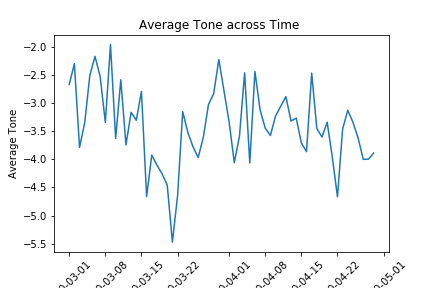
\includegraphics[width=0.49\textwidth]{images/avgtone.png}\label{fig:avg}}
 	\subfloat[GDELT Average Tone 3 Day Moving Average]{  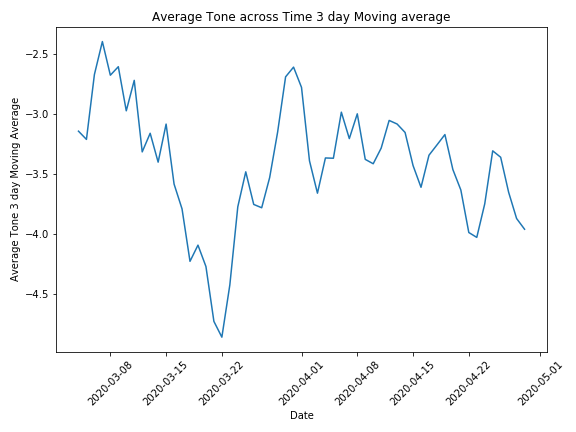
\includegraphics[width=0.49\textwidth]{images/avgtone_ma.png}\label{fig:avg_ma}}\\
 	\caption{GDELT Average Tone over time and Moving Average}
 	\label{fig:avg_tone_diff}
 \end{figure}
 
 Figure \ref{fig:gs_diff} shows the daily average of the Goldstein Scale of events across time, and as with the average tone plots, the 3 day moving average is shown in Figure \ref{fig:gs_ma}. The Goldstein Score, like the Average tone, appears to be chaotic, though in this case it shifts frequently from positive to negative. The moving average shows that there appears to be a peak halfway through the time period, followed by more fluctuation. 
 
 \begin{figure}[H]
 	\centering
 	\subfloat[GDELT Goldstein Scale]{  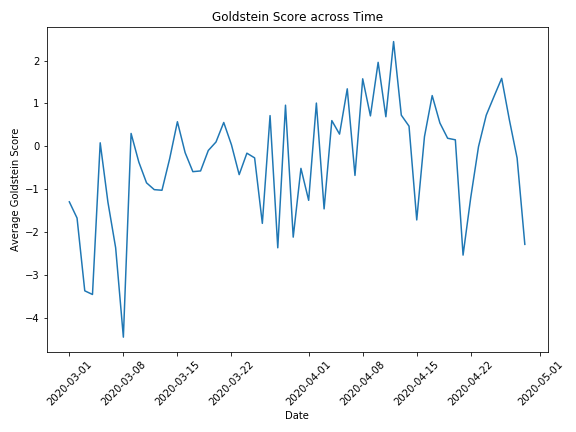
\includegraphics[width=0.49\textwidth]{images/goldsteinscore.png}\label{fig:gs}}
 	\subfloat[GDELT Goldstein Scale 3 Day Moving Average]{  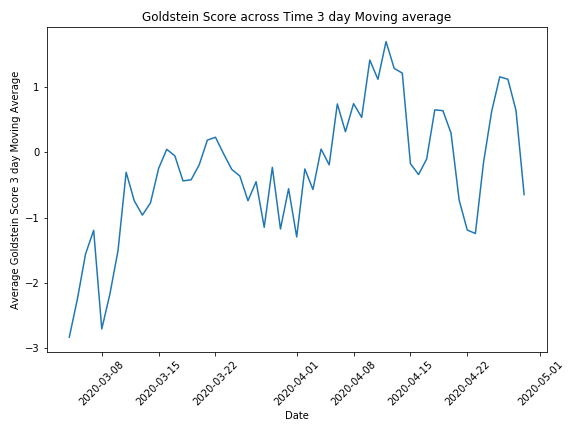
\includegraphics[width=0.49\textwidth]{images/goldsteinscore_ma.png}\label{fig:gs_ma}}\\
 	\caption{GDELT Goldstein Scale over time and Moving Average}
 	\label{fig:gs_diff}
 \end{figure}
 
 
\subsubsection{Stock Market Data}
Stock Market data was acquired from the yahoo! finance United Kingdom website. For the stock market data, the model would predict whether the stock would rise or fall over an entire day. Since there were potentially lots of events occurring on each day, the average was taken of the Goldstein scale and the Average Tone for all events on a specific day. 

Figure \ref{fig:dow_diff} shows the Dow difference between open and close prices on a daily basis. This data is fairly chaotic, with the difference jumping between positive and negative frequently and without an apparent pattern, thus a moving average of 3 days was plotted, which also remains slightly chaotic, but more trends appear. The market difference appears to be getting negatively larger towards the middle of the time period before recovering towards 0. The stock prices appeared to take a dive throughout March, which can be explained by the USA China trade flareups, and more pertinently, the impact of Covid-19. Examining the moving average, the daily difference in the Dow Jones follows a somewhat similar path as the average tone, with a, specifically with a large trough present in the time interval. This trough was present a few days after the average tone trough, as the average tone trough occurred on the 22nd of March, whereas the daily difference trough was on the 24th of the month.

\begin{figure}[H]
	\centering
	\subfloat[Dow Jones Daily Difference]{  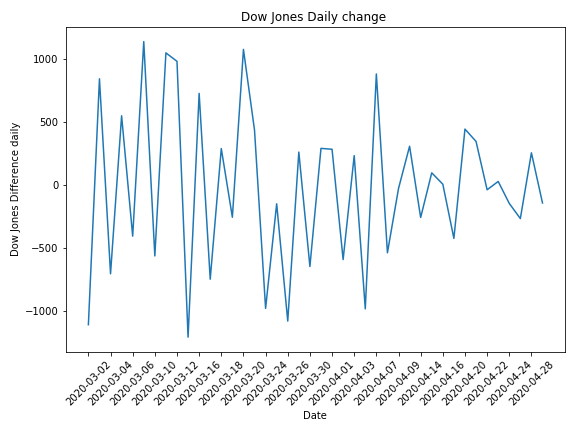
\includegraphics[width=0.49\textwidth]{images/dow_diff.png}\label{fig:diff}}
	\subfloat[Dow Jone Moving Average]{  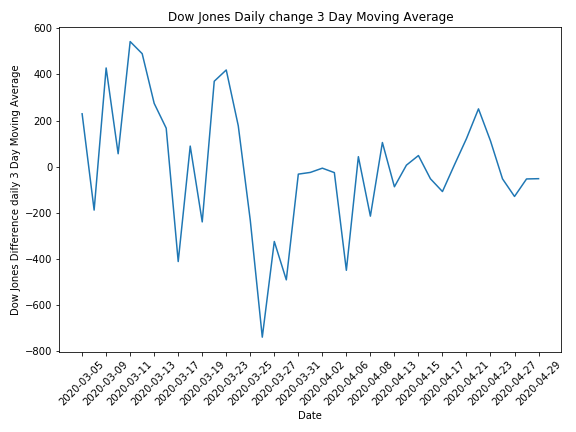
\includegraphics[width=0.49\textwidth]{images/dow_diff_ma.png}\label{fig:dow_diff_ma}}\\
	\caption{Dow Jones Daily Difference and Daily Difference Moving Average}
	\label{fig:dow_diff}
\end{figure}


\subsection{Topic Modelling}
There were several topic models run using several data sources. Firstly, an LDA model was run on a single day's GDELT event data. This was the whole day's worth of data with no country filter applied. This was to examine whether topic modelling was possible for the headlines data.  

The LDA models were applied on the USA/China GDELT data within the interval of the 1st of March to the 30th of April. 

After running the LDA models, the K-Means cluster models were run on the USA/China GDELT data with TF-IDF preprocessing.

\subsubsection{Preprocessing}
%The first topic model was fitted on one day data, using the gensim package. 
All of topic models worked on the basis of using a corpus for the data, This meant that the URLs were parsed, and then headlines taken from them. Each headline was used as a document, and split into the requisite words to be used. In this process the text was cleaned to remove punctuation and special characters, and formatted to build a corpus full of documents, with each document being a list of words from one URL. 
\subsubsection{TFIDF}
The TFIDF vectoriser present in the sklearn package was used to calculate the vector encodings, and was used as the basis of the cluster analysis for K-Means clustering. It was run across the USA/China filtered data to get an initial understanding of which terms would be most important across the dataset. This was then used to numerically transform the headlines for the K-Means algorithm. 

\subsubsection{LDA}
To run the LDA model, the gensim package in the python programming language was used \cite{rehurek_lrec}. Several LDA models were fitted, each with a different number of topics, to examine which would be the best number of topics for the data. After the data was fitted, several phrases were inserted in the LDA model to see the probability of those words being in that topic or not. 

It was found that LDA models were only able to return a probability value for words which were already in the corpus.  This meant that any news headlines which contained \textit{any} word not originally in corpus would not be able to be accurately classified by an LDA model. This meant that this type of model could not be used to separate and filter irrelevant headlines from those headlines which were focused on the headlines in the model. 

\subsubsection{K-Means}
K-means clustering was also fitted on the data. The package used was the K-Means clustering algorithm already implemented in the sklearn python package. Several cluster numbers were tried, from fitting with 2 centroids to fitting with 4 centroids. The Mahalanobis distance and the euclidean distance was calculated for each clusters' points. Furthermore, sample phrases were tested against K-Means models, to see if the cluster was meaningfully able to recognise the difference between words related to the clusters and noise in the algorithms. From an implementation perspective, a random seed was set for each of the clusters so the centres would start at the same point, and thus the results would be reproducible. 

To test the efficacy of the models with regards to filtering data, the Mahalanobis distance was calculated for each of the clusters for a selection of phrases. These phrases were varied in length and content. Some of the phrases were relevant to the main topics/content of the topic models,  namely related to the pandemic, or the USA or China, such as the phrase `coronavirus hits remote utah`. Other phrases were completely unrelated to the topic models such as 'the nikkei closes 90 points down` and `aboriginal peoples australia complain`. A full list of phrases is shown in appendix \ref{phrases}. If the cluster models were accurate in filtering information, the phrases closer to the topics at hand would be physically closer to the clusters in p-dimensional space and thus have smaller Mahalanobis distances than phrases which weren't close to the topics in hand.  

\subsection{Stock Modelling}
The main aim for this type of modelling was to predict whether the stock shifted up or down over the course of a day. Each day's difference was calculated between the opening and closing prices, and either a 1 or a 0 was used to represent the stock market going up and down. For the scope of the project, and similar to other modelling approaches, it was decided to only predict either the market going up or down. There were several models which were tried, detailed in \ref{models}. In all cases the response variable being predicted is the change in the stock price over a day. This takes a value of 1/0 for either a fall or rise. This is denoted Y at time t ($Y_{t}$), where t is a day, and ordered 1 to T, for the time interval used for training the model (April 1st to May 31st 2020). The predictors used were the Average Tone and Goldstein scale values for each day, along with differing amounts of predictors for previous day's data.

All of these models were tested and ranked on their accuracy. This was a percentage of the number of days that the model predicted whether the stock went up or down correctly. The `best` model was selected to be the one which had the highest accuracy values. The best model was then used to predict the stock shifts for the days between the 1st of May and the 30th of June, on the same set of data, i.e. the USA China GDELT filtered data. 

Another measure of the validity/accuracy of the best model was comparing it to a reference model. This reference model would be of the same model type as the final model, but only use the previous day's stock shift, and \textit{not} the Average Tone or the Goldstein Scale values for as a variable used for prediction. The aim with this reference model was to see if the Average Tone and/or the Goldstein Scale actually provided any extra information and insight into the stock market to a model compared to a model which just used the previous day's stock shift.  

\subsubsection{Preprocessing}
There was substantial preprocessing required for the data, first of all the stock market does not open on weekends or other holidays, however news and events do. Thus, the news over weekends was collated and averaged into the Friday figures. This meant that the prediction data had to the shifted, to ensure that information from the future was not being used to predict the data.

The next issue to consider whilst preprocessing the data was the issue of lag modelling. It is reasonable to expect that if there is an underlying relationship between the Goldstein Score/Average Tone and the stock price, a specific day's stock price changes would not restricted to just the previous day's news, but instead could be impacted by news over the previous several days. Thus the average scores and the Goldstein scales would have to be smoothed using several moving window calculations.

\subsubsection{Models}
\label{models}
All of the models tried were classification models, as by reducing the stock price changes into up or down, it became binary data. There were 4 main models which were tried, a Naive Bayes model, a Random Forests Model, a Support Vector Machine, and a simple Logistic Regression. Furthermore, a simple multi layer neural network was also tried on the data to see if there was any underlying representation that could be learned. All of the models were trained using 3 predictors, the Goldstein Score and the Average Tone of each day's events, and the previous day's stock change. 

Initially simple models were fitted with no averaging or smoothing of the predictors performed. However, it was assumed that an individual event could affect prices for several days, thus the Goldstein scale and Average tone predictors were smoothed using several different kinds of moving windows. There were 3 different moving window types tried, firstly a simple average was taken where each day was weighted evenly. The second method of moving window was an exponential decay window, and similarly a half Gaussian moving window. The moving windows were all spread over three days, as it was felt that this would provide the best balance at weighting past events evenly, without diluting the effect of the most recent news.

To test whether the previous N days' stock shift affected a specific day, three extra predictors were added, these predictors, along with the previous day's change, represented the stock shift for each of the previous four days. These were used alongside the unsmoothed Average Tone and Goldstein Scale values to predict the stock prices. These models are henceforth referred to as the Manually Lagged Models.

All of these models were trained and tested on the March-April data, and the results are reported in chapter \ref{results}.

To both show how this sort of predictive model would be used in the real world, and to test the `best` model's predictive capacity in `real` time, the `best` model was used to build a simple portfolio. For time reasons this only consisted of a single stock, where shares were bought or sold on a daily basis based on the model's confidence in the following day's stock shift. This was to mimic the behaviour of being used in real time, where there would only be new news for the current day, and based on the previous news and each day's news, the next day's prediction would be made. The stock chosen was Apple Inc.\ as this stock had the highest weighting in the Dow Jones index. The Apple historical data values were also procured from the finance Yahoo United Kingdom website. 

This was a very simple portfolio test, where each day's prediction triggered buying and selling of the stocks, i.e. stock was only ever held when the confidence of market shift was not above a threshold, otherwise stock would be bought and sold daily. There were several hyperparameters involved, namely these were the initial capital, initial number of shares, the confidence threshold required to trigger buying or selling stocks. There were also two additional hyperparameters, these variables controlled the fraction of capital used to buy stock, or the buy-factor, and the fraction of stock to sell at any given point, sell-factor. These variables were constant for every run, so for one test on the May to June time period, every time the confidence in the prediction for the next day was greater than the confidence threshold, and the market was predicted to increase, the buy-factor amount of the capital at that point was used to `purchase` stock. The reverse happened when the market was projected to decrease, with the sell-factor fraction of the stock being held being sold. Since geopolitical events can occur after the market close which are factored in by the predictive model, the stock close price was used as the reference price for buying and selling stock. 

For the May to June time period, the number of shares, and the capital was tracked, along with the total asset value, which was the total capital plus the monetary value of those shares at the closing price each day. Three different strategies were used, one which would maximise the shares by using more capital to buy shares, one which would maximise capital by minimising the number of shares held at any point, and one which would be in the middle of those two strategies.

The `best` predictive model's portfolio was also compared to a portfolio which used the reference model, and the results are shown in chapter \ref{results}.

\section{Results}
\label{results}
\subsection{Topic Modelling}
\subsubsection{TF-IDF}
The top TF-IDF terms are shown for the USA China data across the corpus in Figure \ref{fig:tfidfusachina}. This data was achieved by taking the average of the TF-IDF values across the entire dataset. The average values are slightly lower across the corpus compared to individual documents, as there will be a number of documents where specific words have TF-IDF values of 0, as those words do not exist in those documents. These 0 TF-IDF values are included in the mean calculations as the parsing process for URLs is not perfect in retrieving headlines. If the 0 TF-IDF values were excluded from the averaging calculations, the top words by TF-IDF would be non representative of the whole corpus, as there may be some `words` present only in a small number of documents, where the words are the result of parsing errors, and thus have artificially high TF-IDF values if their 0 values from all other documents are not averaged.

\begin{figure}[H]
	\centering
	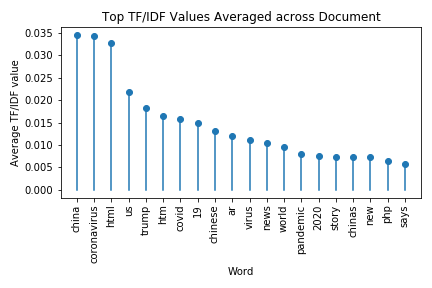
\includegraphics[width=0.8\textwidth]{Images/usa_stem_tfidf.png}
	\caption{Plot of the top 15 words which used TF-IDF in the USA/China specific data}
	\label{fig:tfidfusachina}
\end{figure}

Perhaps as expected, the most important and often occurring words are China and coronavirus.  Amongst the top words are also US, and Trump, along with variations of China and covid-19 and references to the pandemic. This is most interesting as a result, as something which no one had heard of prior to January/February dominated the news in March and April.

One of the other main words which pops up is html. This is most likely as a result of the fact that most of the URLs end with `.htm` or `.html`, and during the parsing html gets treated as a commonly occurring word. It was not removed as there could be legitimate stories which have the word in them. 

For the top values, the distribution of the tf-idf values across documents was calculated, excluding the 0 values. This is shown in Figure \ref{fig:tfidfdist}. The distributions are different to each other, but both follow a similar pattern in having a centre of the distribution be around a Tf-IDF value of around 0.25. One of the notable exceptions to this is the word `ar`, which is another error as a result of parsing. World and news both have a spike later on, but that is most likely due to the smaller sample size.

\begin{figure}[H]
	\centering
	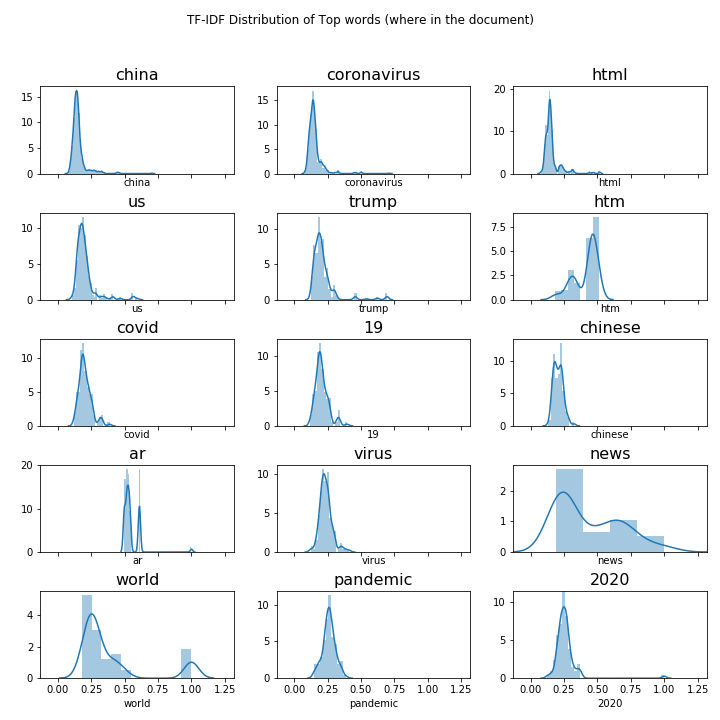
\includegraphics[width=0.8\textwidth]{Images/usa_tfidf_top_distribution.png}
	\caption{Distribution of the TF-IDF values across documents of the top 15 words (excluding documents where the Tf-IDF value was 0)}
	\label{fig:tfidfdist}
\end{figure}

\subsubsection{LDA}
\paragraph{Initial LDA}
Initially a topic model was run on one day's worth of Event data. The day was the 1st of November 2019. This was done as a reference point before running the LDA models on the specific USA/China chosen data.

There were two different topic models tried. Firstly one model with 3 topics was tried and then one model with 5 topics. It was unknown how many topics would be present in the data, thus two different values were chosen, one with a smaller number of topics (3), and a slightly larger number of topics (5). The two values were tested to see if a smaller or a larger number of topics would represent any topics present in the data. The top words from each model are shown in word cloud format in Figures \ref{fig:single3wc} and \ref{fig:single5wc}. Alongside the word cloud, for each topics, the weight and the word count of the top words was also calculated and plotted. 
	
\begin{figure}[H]
	\centering
	\subfloat[Word Cloud 3 Topics]{  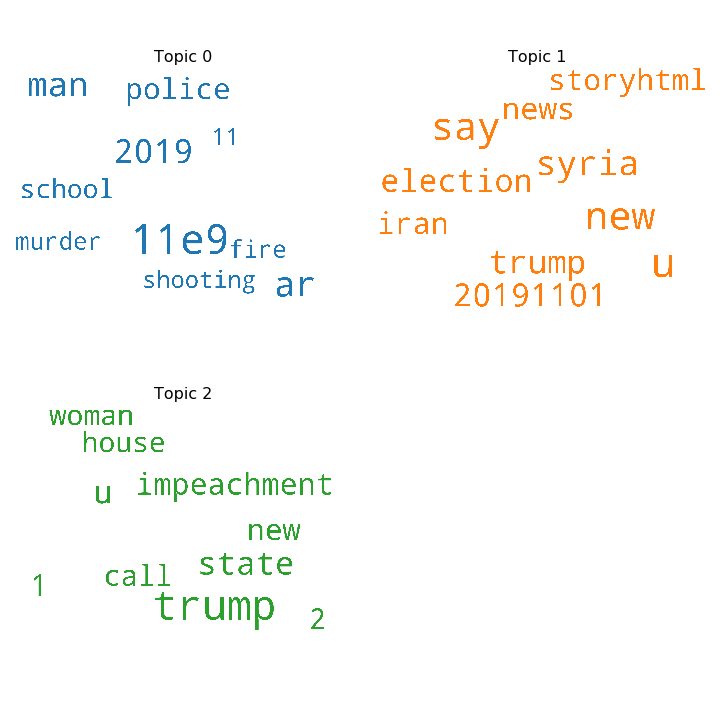
\includegraphics[width=0.8\textwidth]{images/single/word_cloud_single_3_topics.png}\label{fig:single3wc}}\\
	\subfloat[Word Weights 3 topics]{  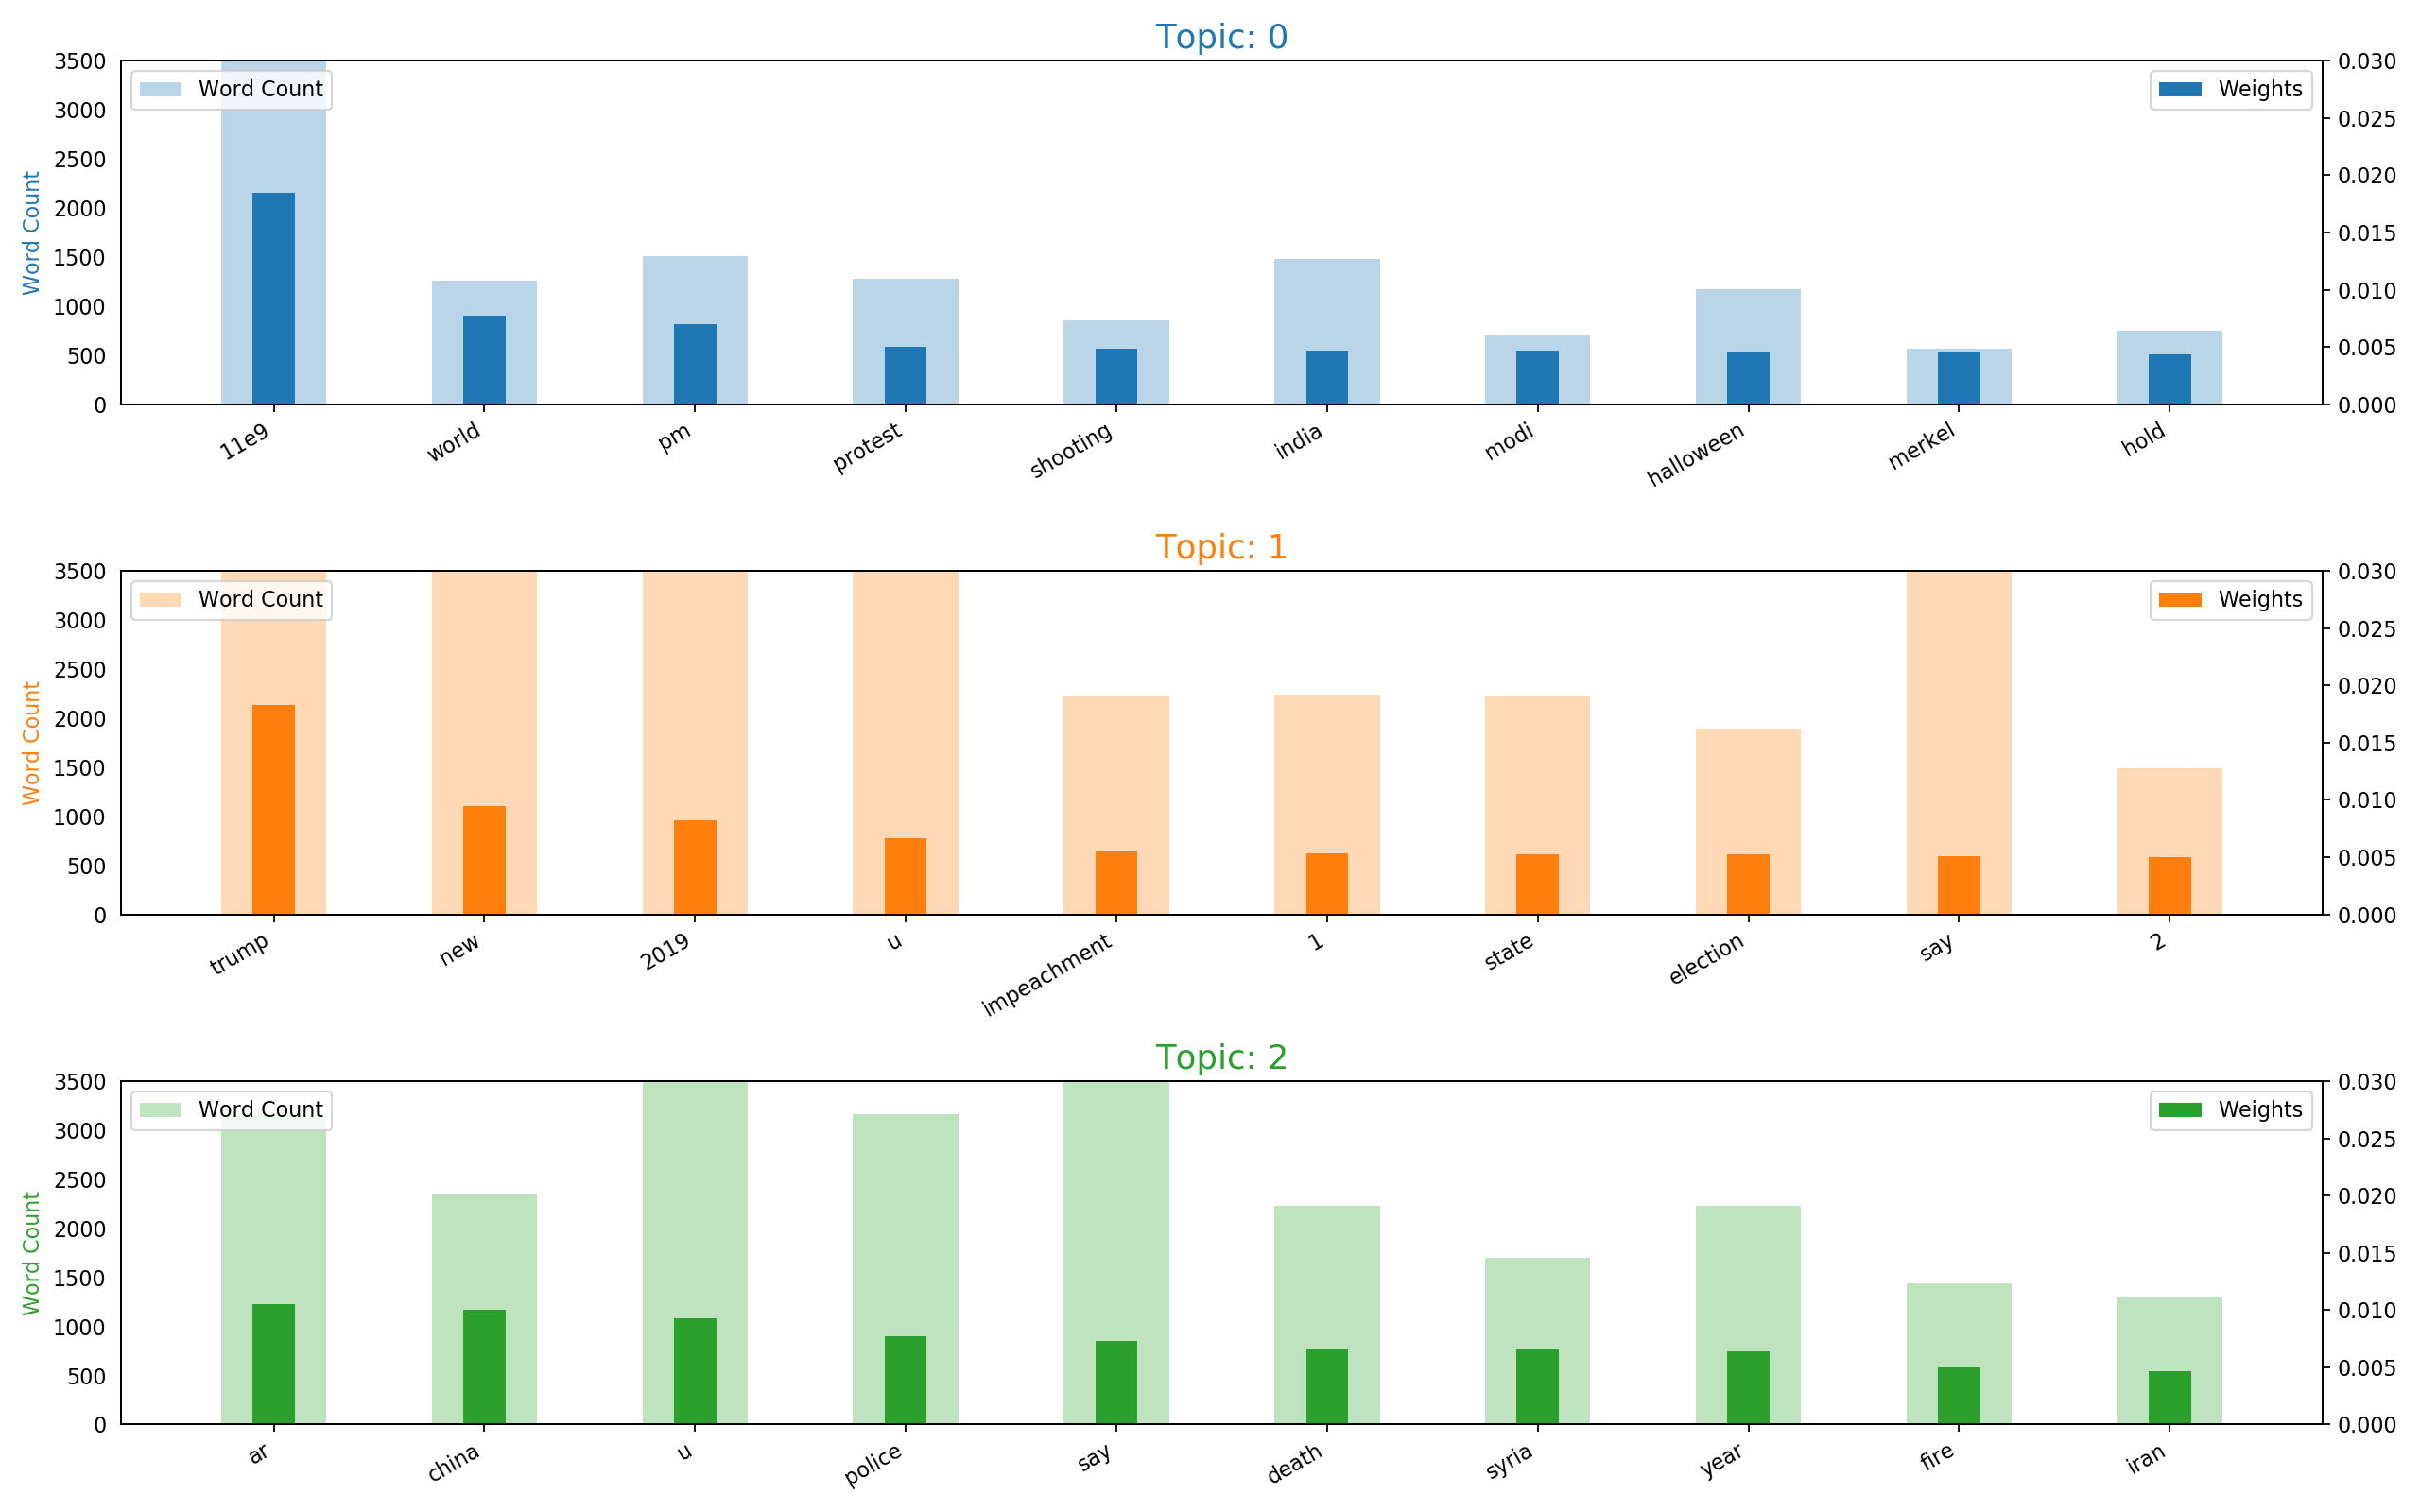
\includegraphics[width=0.8\textwidth]{images/single/word_weights_single_3_topics.png}\label{fig:single3ww}}\\
	
	\caption{Single Day Word Clouds and Word Weights for 3 topics}
	\label{fig:single3}
\end{figure}

Examining the word clouds for the model with three topics, there are not any clear topics which are apparent. Topic 2 could vaguely be about the impeachment process for Donald Trump, Topic 0 appears to be focused on police brutality as a topic, and Topic 1 could broadly be referred to in terms of international news. Examining the word importances, the main theme across topics ia that the word count is not the same as the word importance, in that some words have much higher occurrences, but lower weights and vice versa. This is perhaps to be expected, as the word count and importance do not have to be linked.

\begin{figure}[H]
	\centering
	\subfloat[Word Cloud 5 Topics]{  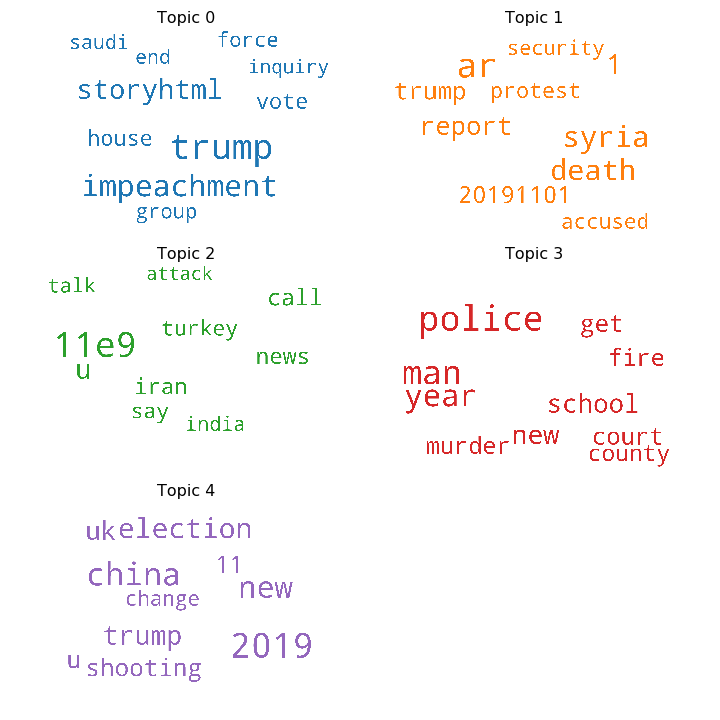
\includegraphics[width=0.8\textwidth]{images/single/word_cloud_single_5_topics.png}\label{fig:single5wc}}\\
	\subfloat[Word Weights 5 topics]{  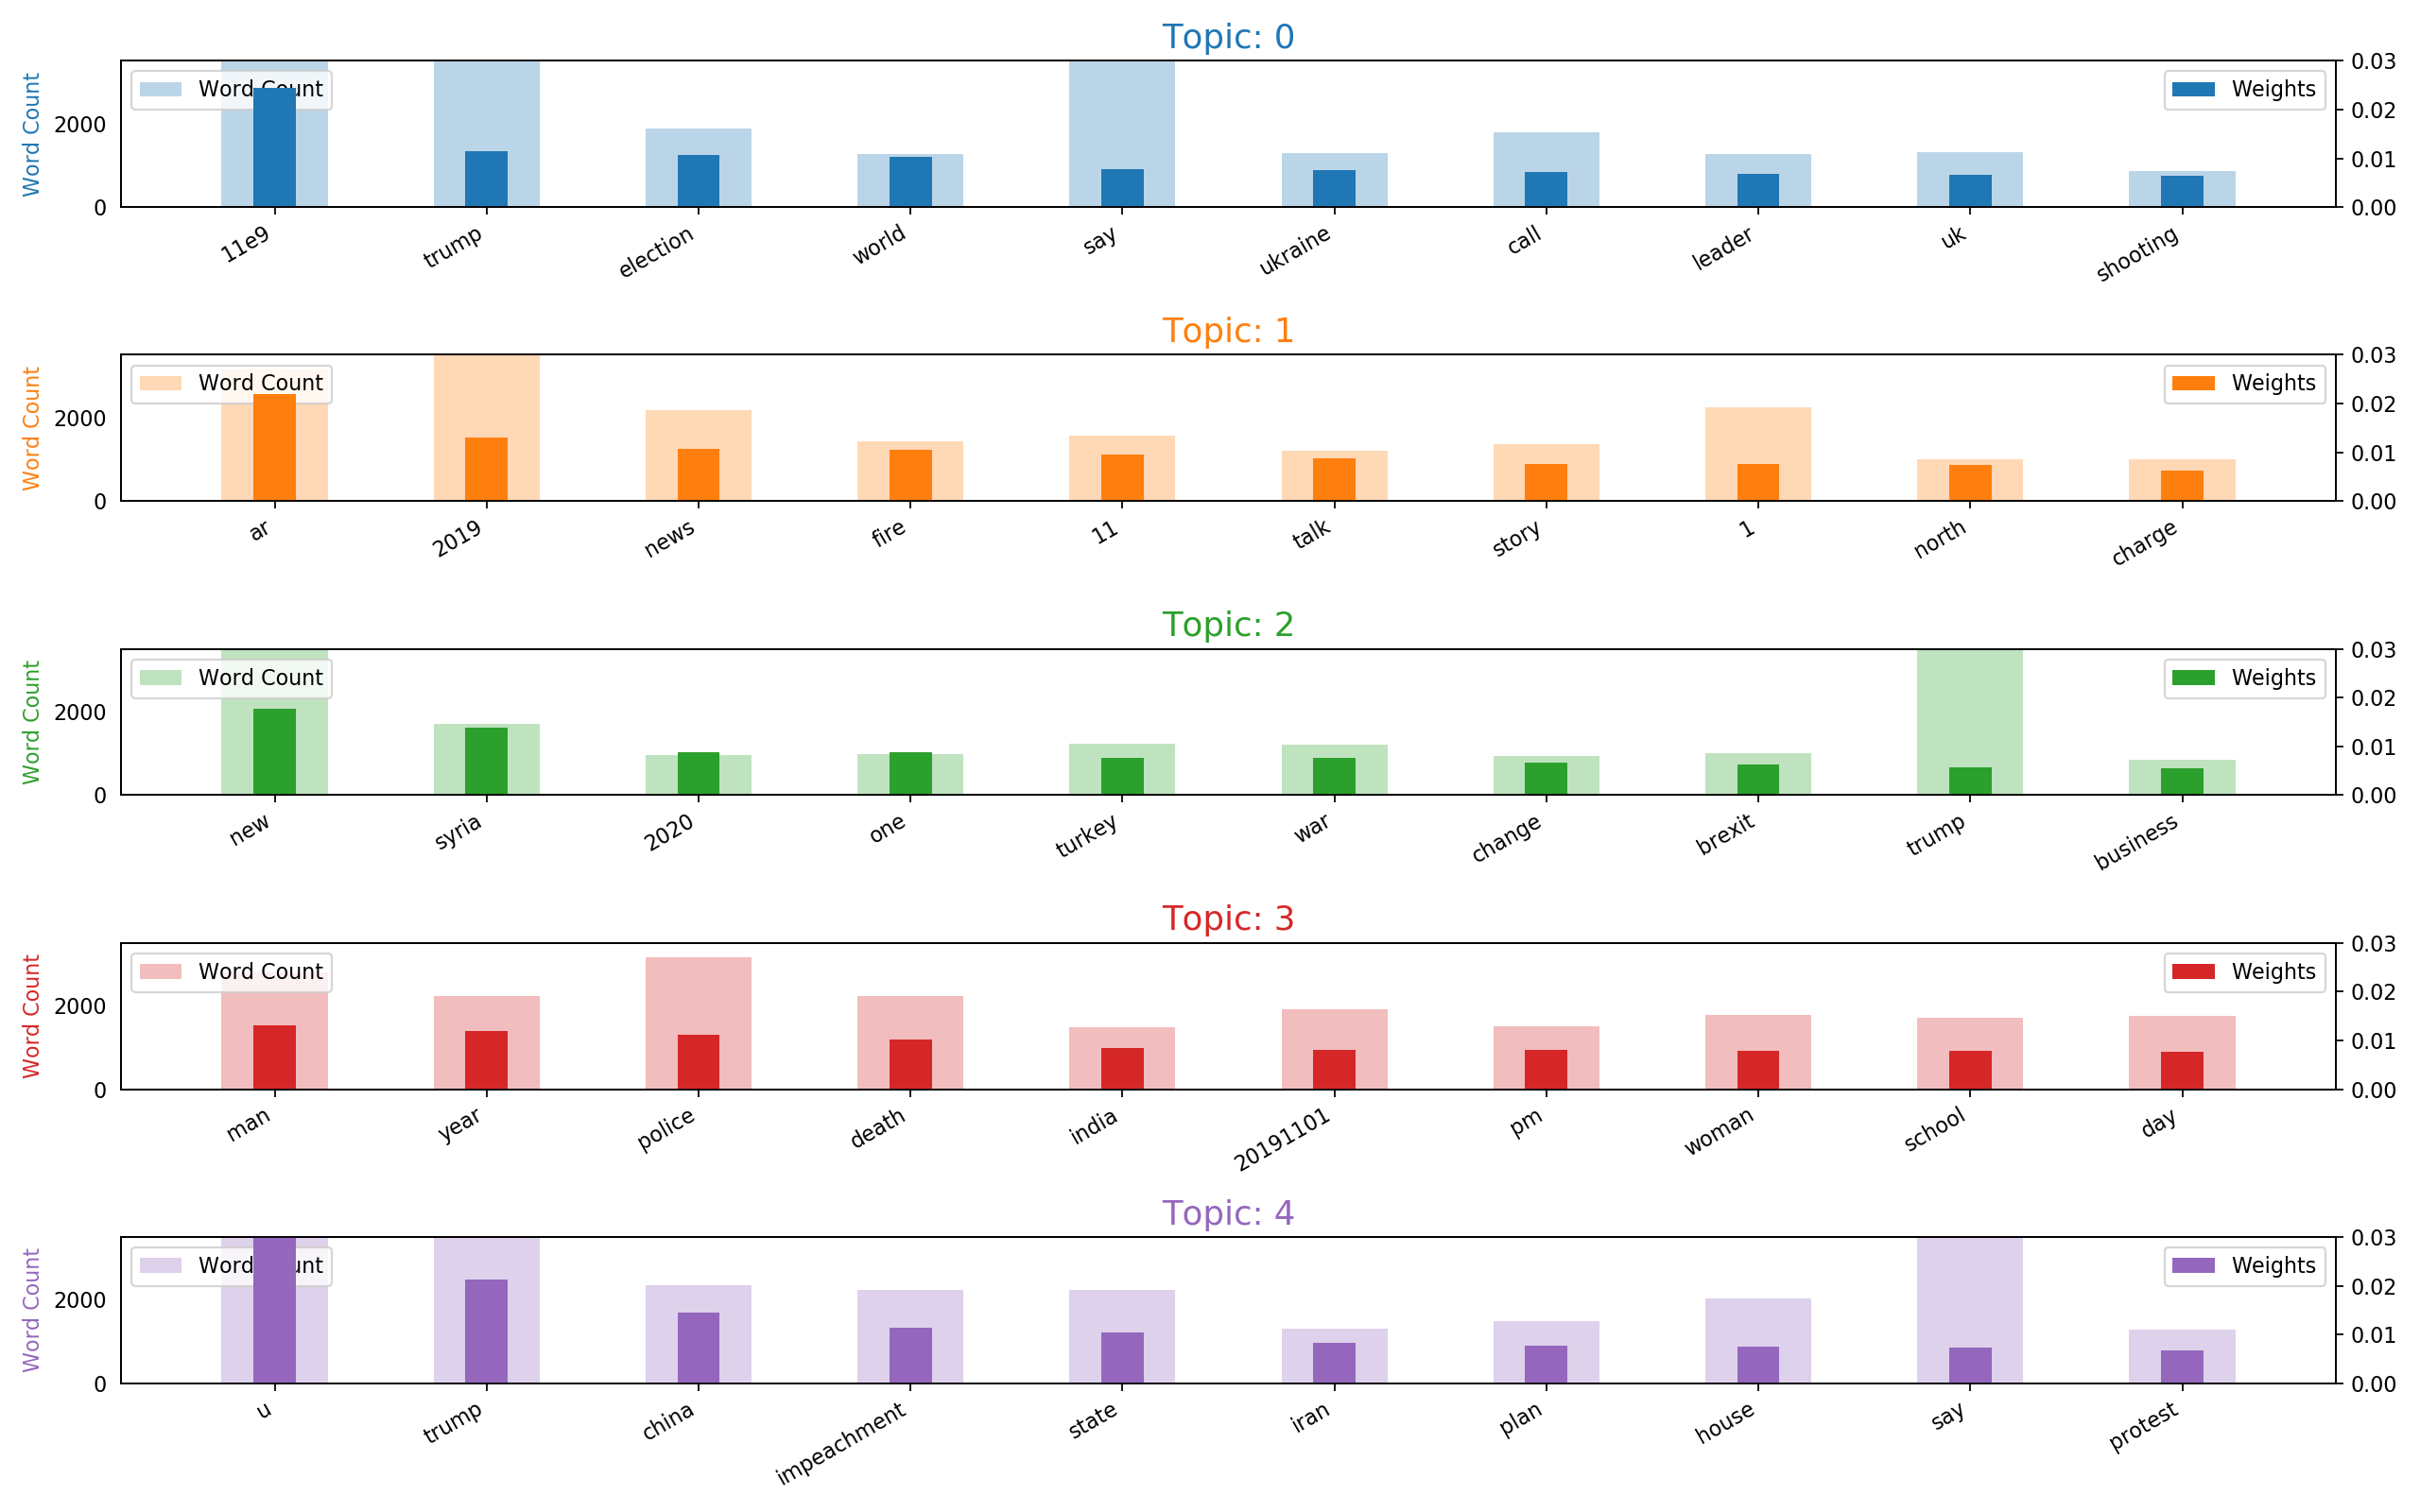
\includegraphics[width=1\textwidth]{images/single/word_weights_single_5_topics.png}\label{fig:single5ww}}\\
	
	\caption{Single Day Word Clouds and Word Weights for 5 topics}
	\label{fig:single5}
\end{figure}	

Examining the 5 topic model, the topics are much closer together, its very difficult to find a central topic for each topic, Topic 3 could potentially be about police and court information, but aside from that there does not appear to any coherency otherwise, with words like Trump being in multiple topics and international countries spread across topics. The word importance and weight plot also does not reveal anything new, like the previous model, the word's count is not related to the importance and perhaps expectedly, the words in the topics are not related to each other.

\paragraph{USA/China Data}
A similar procedure was used for the USA/China data, but models with 2, 3, and 4 topics each were tried, as it was not completely clear whether a smaller or larger amount of topics would represent the data better. The word clouds of the results and the subsequent word importances to each topic are shown in Figures \ref{fig:usa2}, \ref{fig:usa3}, and \ref{fig:usa4}. 
\begin{figure}[H]
	\centering
	\subfloat[USA/China Word Cloud 2 Topics]{  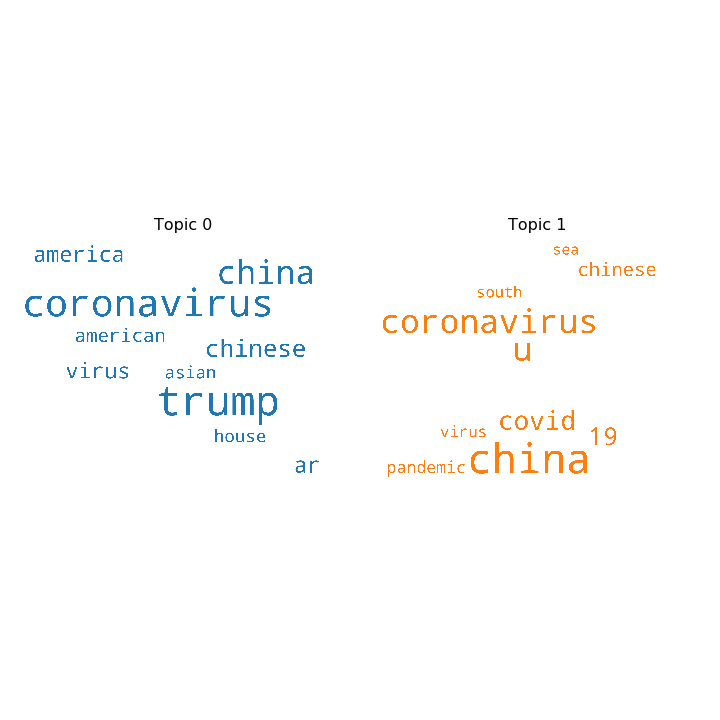
\includegraphics[width=0.6\textwidth]{images/uschina/word_cloud_usa_2_topics.png}\label{fig:us2wc}}\\
	\subfloat[USA/China Word Weights 2 topics]{  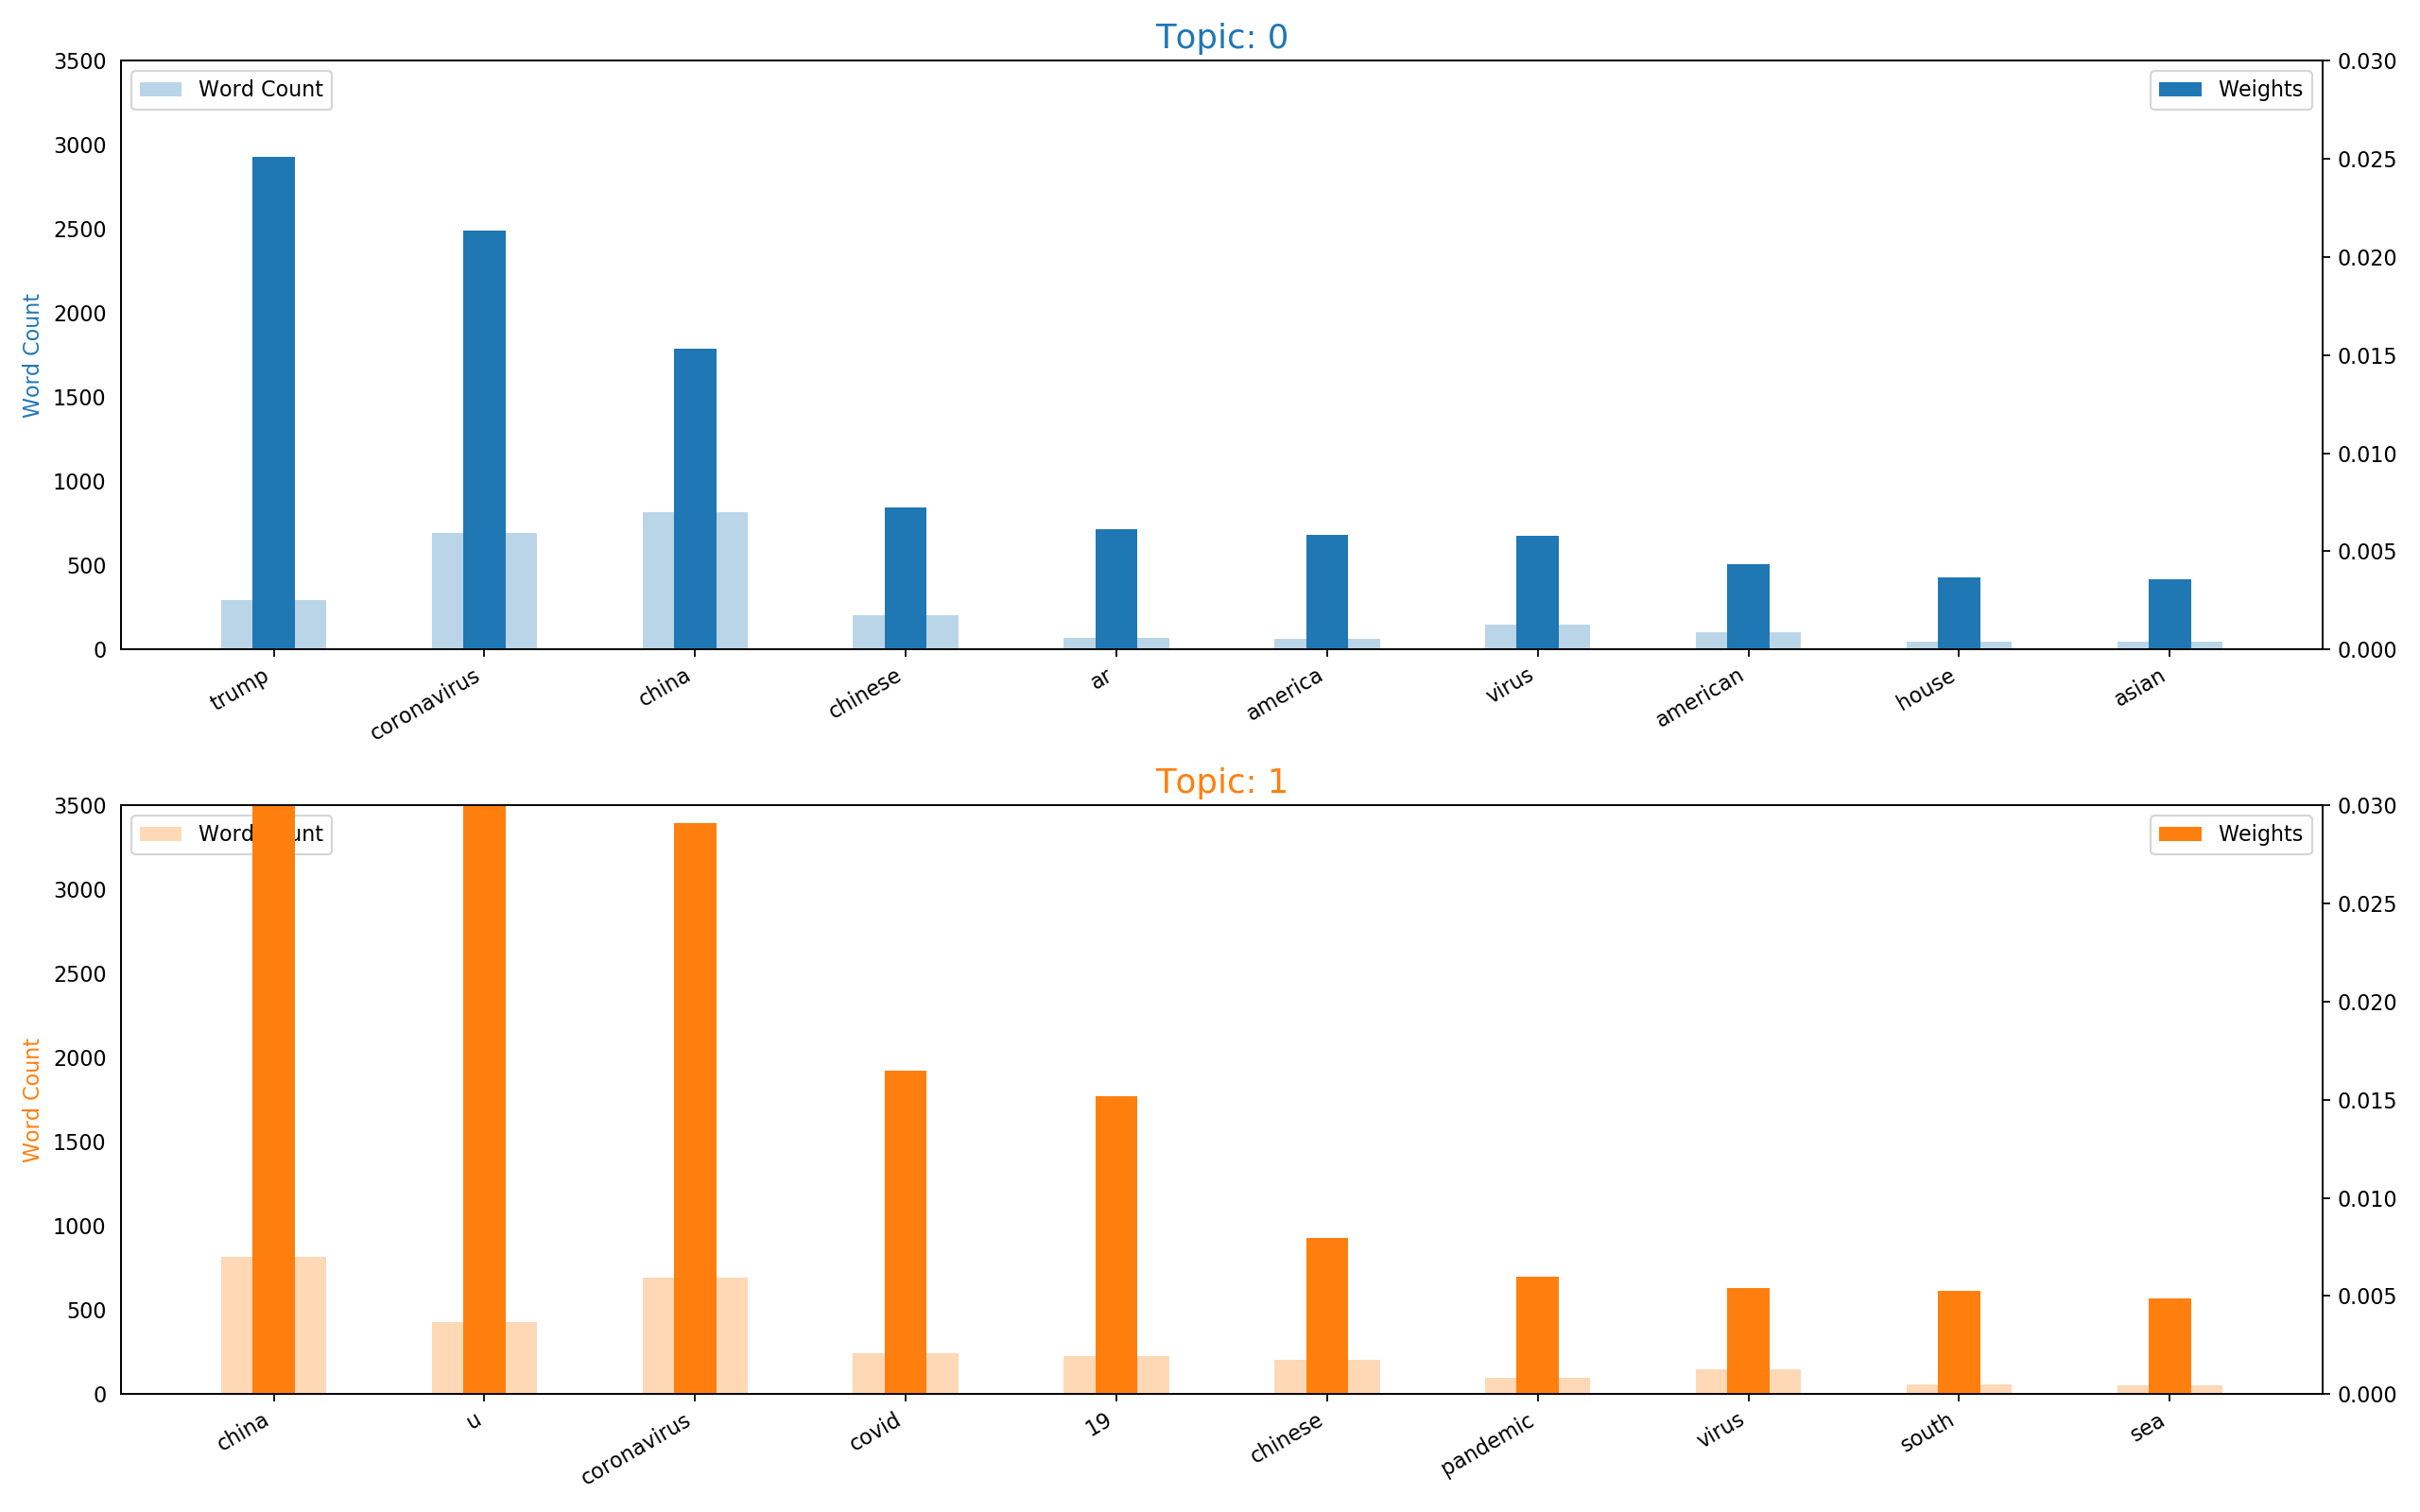
\includegraphics[width=0.8\textwidth]{images/uschina/word_weights_usa_2_topics.png}\label{fig:us2ww}}\\
	
	\caption{USA/China Word Clouds for 2 topics}
	\label{fig:usa2}
\end{figure}
Examining the first LDA model which had 2 topics on the USA China data, the themes are very similar. Words related to the pandemic, and words such as China and Trump appear in both topics, which suggest the model has not been effective in differentiating between the topics effectively. Looking at the word weights in Figure \ref{fig:us2ww}, for all of the words, the weights are all higher than the word counts. The highest word weights by topic are Trump, Coronavirus, China for Topic 0 and China, Coronavirus, and `U` for Topic 1 . `U` appears appears to be another issue with the parsing.  
\begin{figure}[H]
	\centering
	\subfloat[USA/China Word Cloud 3 Topics]{  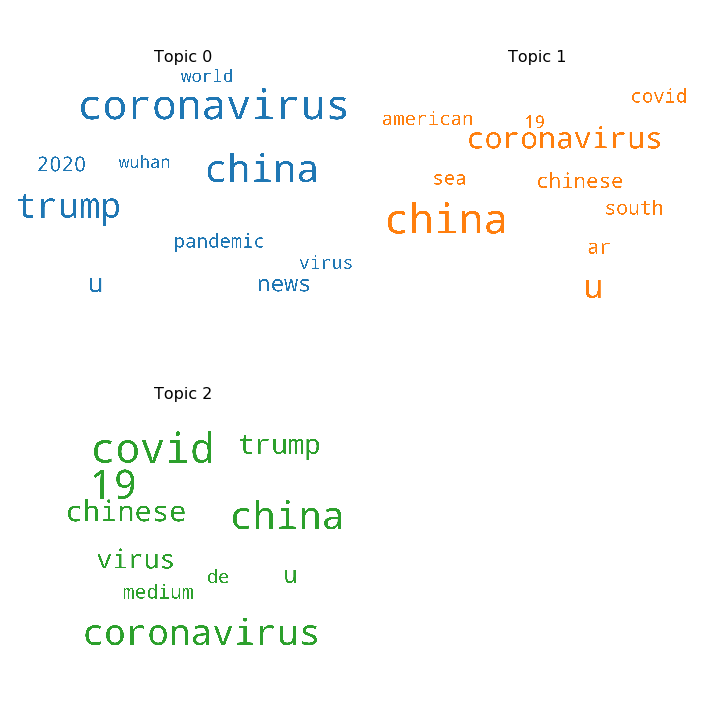
\includegraphics[width=0.6\textwidth]{images/uschina/word_cloud_usa_3_topics.png}\label{fig:us3wc}}\\
	\subfloat[USA/China Word Weights 3 topics]{  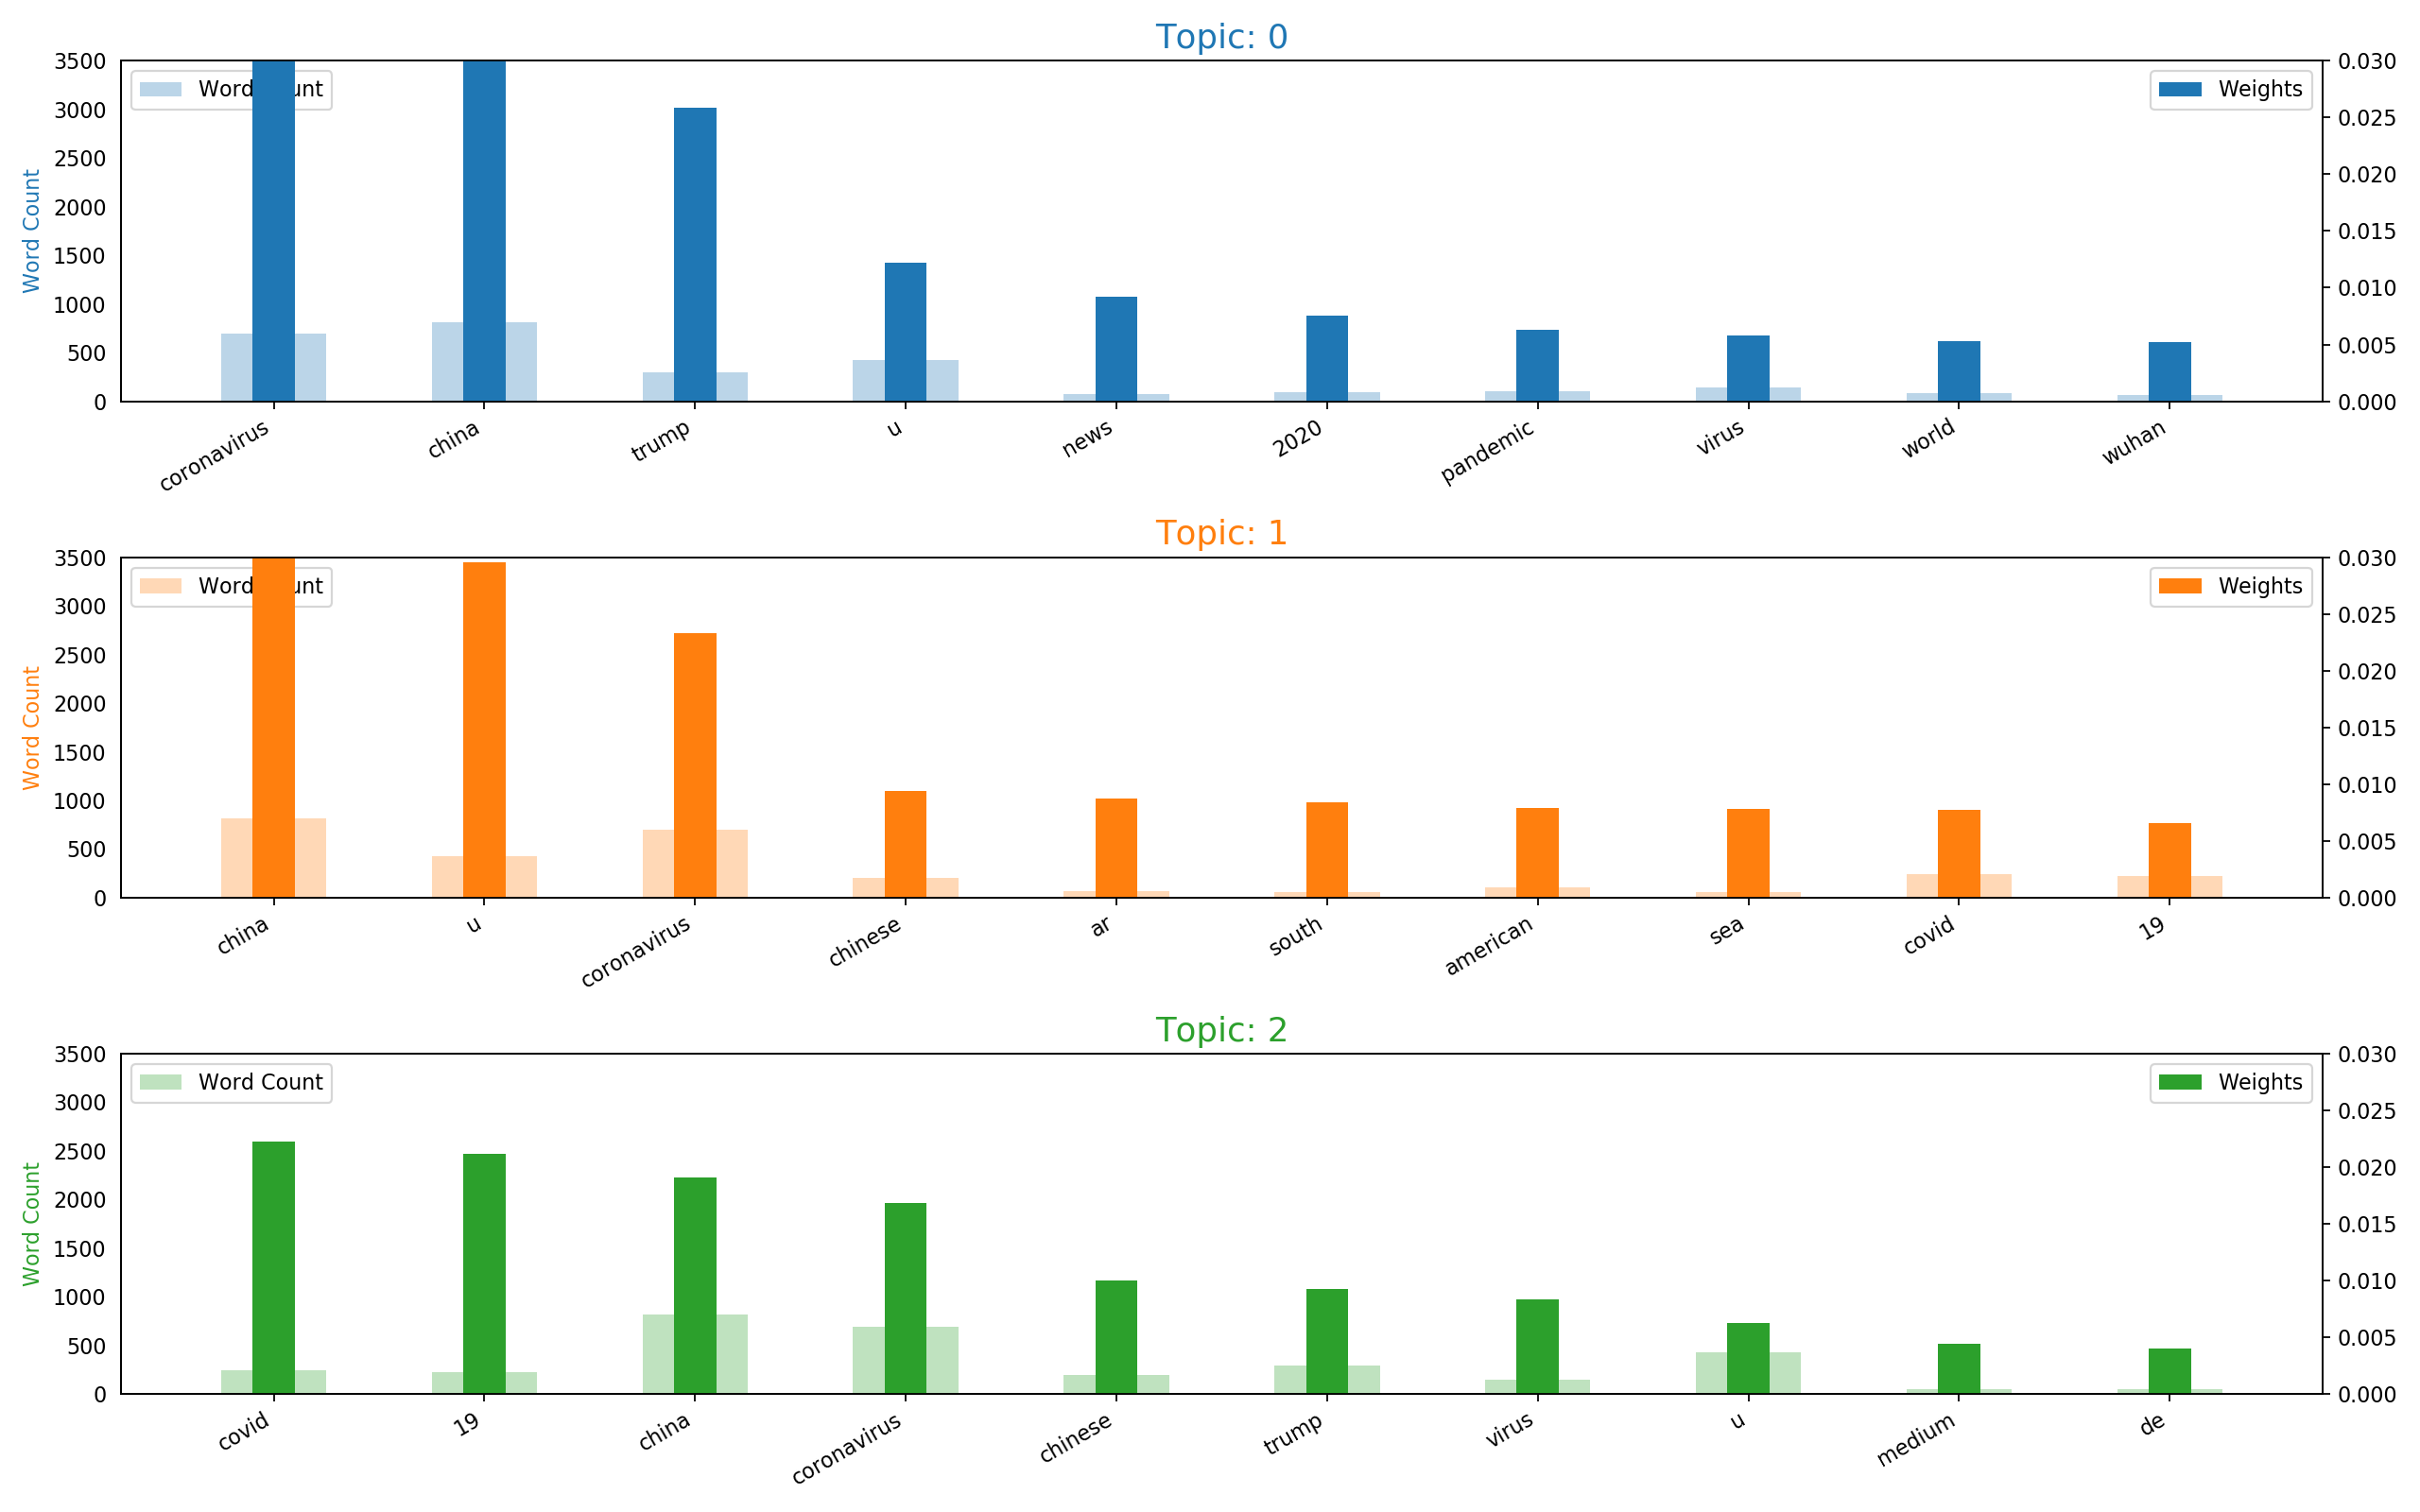
\includegraphics[width=0.8\textwidth]{images/uschina/word_weights_usa_3_topics.png}\label{fig:us3ww}}\\
	
	\caption{USA/China Word Clouds for 3 topics}
	\label{fig:usa3}
\end{figure}

Looking the the three topic model, the topics are even closer together than the two topic model. The main words as before appear in all of the topics, suggesting the topic model hasn't separated any topics well. The word weights are also similar to the two topic model. One of the differences between the two topic and the three topic model is the 3rd topic weights are noticeably smaller than the first and second topics. 

\begin{figure}[H]
	\centering
	\subfloat[USA/China Word Cloud 4 Topics]{  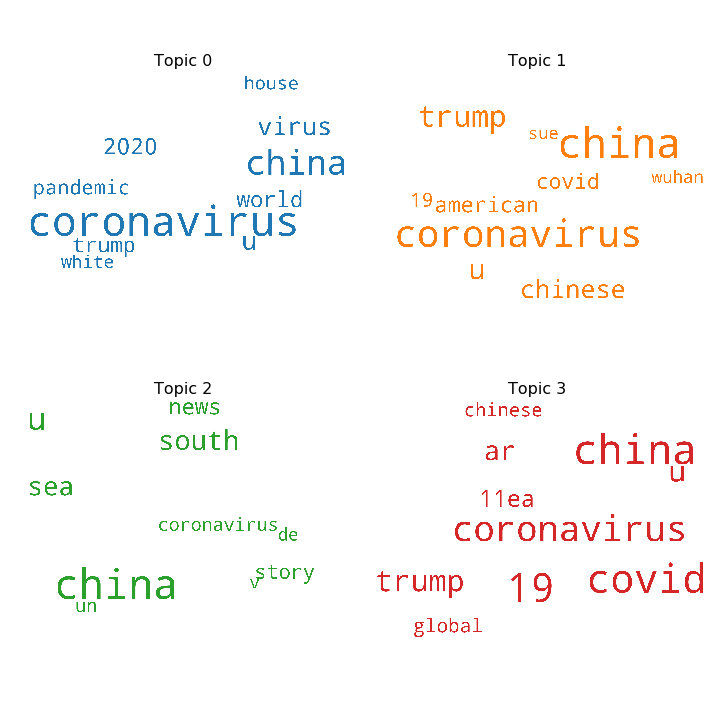
\includegraphics[width=0.6\textwidth]{images/uschina/word_cloud_usa_4_topics.png}\label{fig:us4wc}}\\
	\subfloat[USA/China Word Weights 4 topics]{  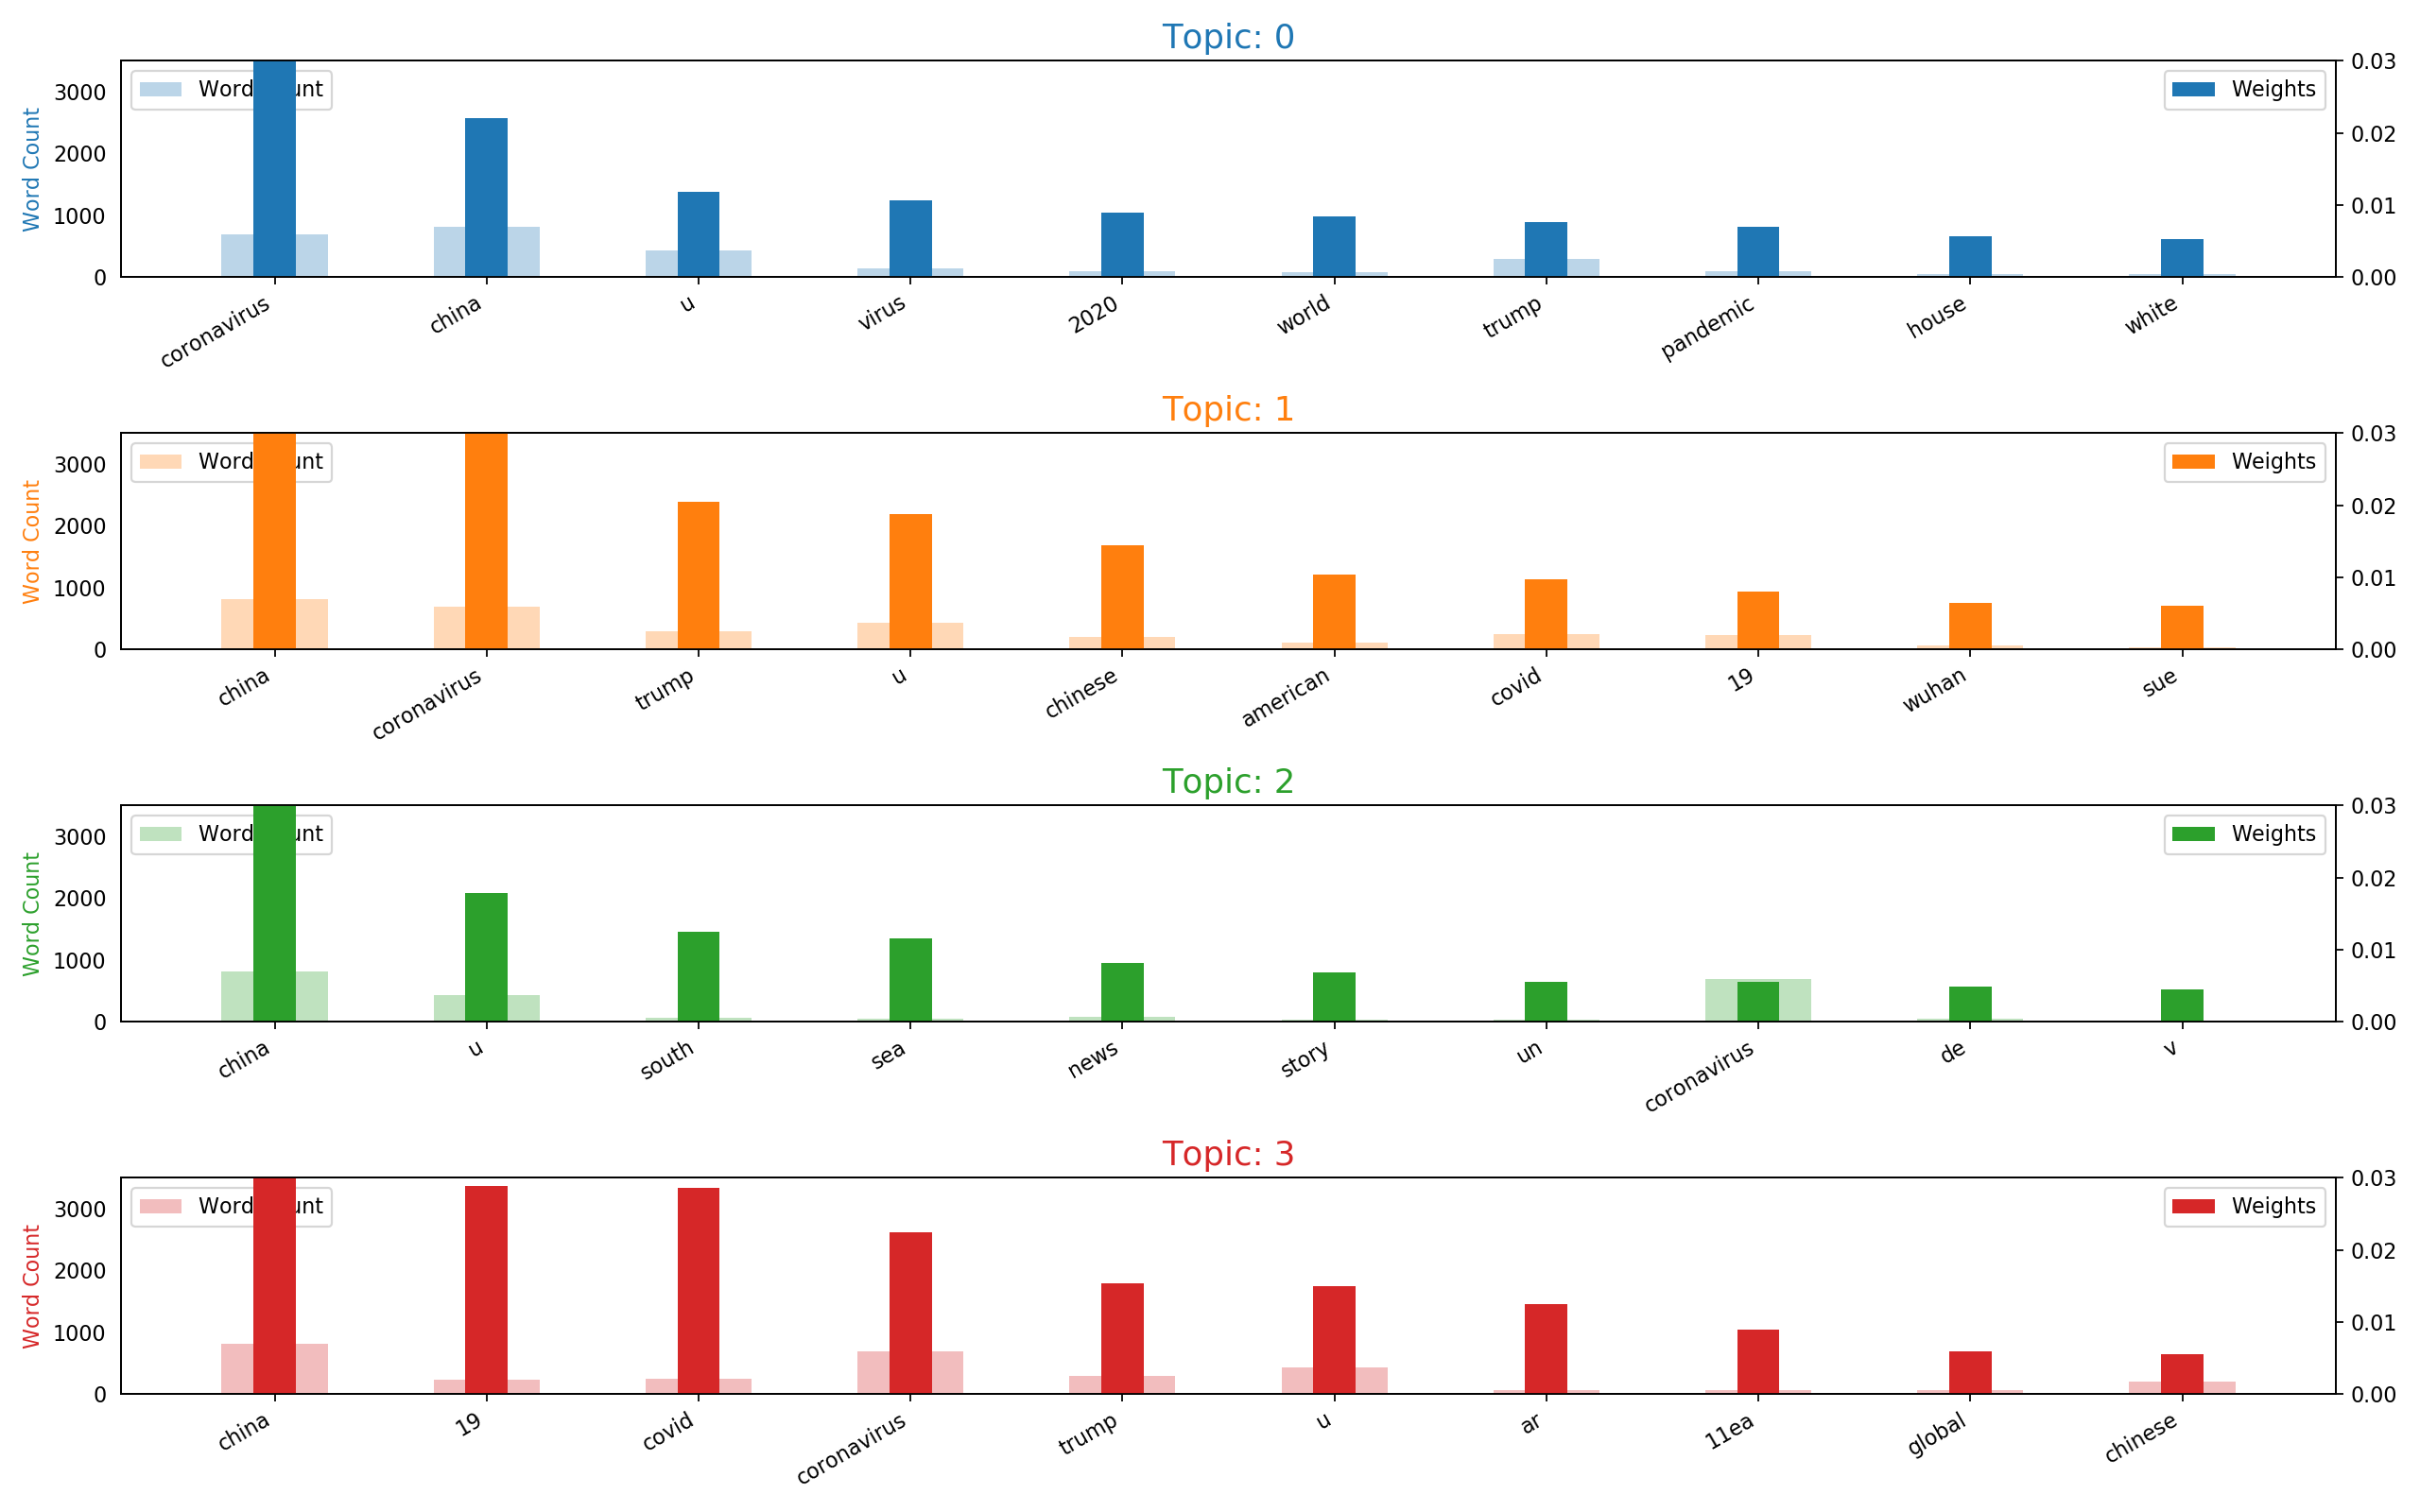
\includegraphics[width=0.8\textwidth]{images/uschina/word_weights_usa_4_topics.png}\label{fig:us4ww}}\\
	
	\caption{USA/China Word Clouds for 4 topics}
	\label{fig:usa4}
\end{figure}

The 4 topic model behaves in a similar manner to the previous 2 topic models. the main words are split across the 4 topics with no real distinction between the topics present. 

\subsubsection{K Means}
Similar to the LDA models, the K-means was tried with 2, 3, and 4 clusters. The word cloud of the top words are shown in Figures \ref{fig:wck2}, \ref{fig:wck3}, and \ref{fig:wck4}. Alongside the word clouds, the clusters were decomposed into 2 and 3 dimensions by both Principal Component Analysis (PCA) and T-distributed Stochastic Neighbour Embedding (T-SNE) \cite{maaten2008visualizing}. This was to see whether the clusters had been successful in separating the data at any level. This is shown for the different number of cluster in Figures \ref{fig:k2pca}, \ref{fig:k3pca}, and \ref{fig:k4pca} respectively. Furthermore, the Mahalanobis and Euclidean distances were plotted for all of the points associated with a cluster for all of the clusters present. This is shown in Figures \ref{fig:distk2}, \ref{fig:distk3}, and \ref{fig:distk4} respectively. 

To compare the efficacy of clusters in being able to filter information, the Mahalanobis distance from centre of clusters for variety of phrases as calculated, and plotted in Figures \ref{fig:wordsk2}, \ref{fig:wordsk3}, and \ref{fig:wordsk4}, alongside the distribution of points for each cluster. For all of the Mahalanobis distances, the phrases were several orders of magnitude out from the distribution of points for each cluster, so the Mahalanobis distance results were logged before being plotted.  
\paragraph{Clustering with k=2}
\begin{figure}[H]
	\centering
	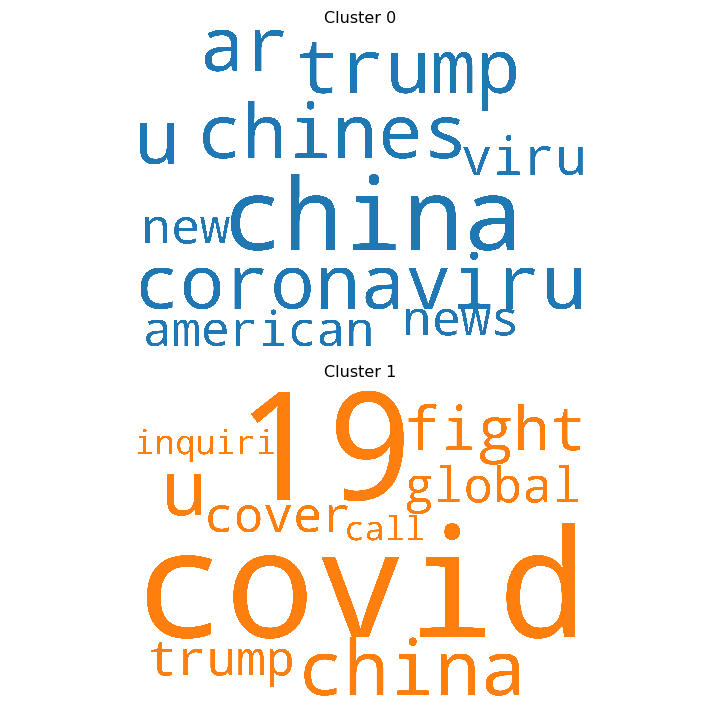
\includegraphics[width=0.8\textwidth]{images/kmeans_word_cloud_k=2.png}
	\caption{Word Cloud for k=2 clusters}
	\label{fig:wck2}
\end{figure}
Examining the word cloud created for a two cluster model, a similar picture appears as with the LDA models. There are several words which are close to both of the clusters, which, in a similar fashion to the LDA model, mean that any topics present are not being differentiated. This is evident in Figure \ref{fig:k2pca}, in which both T-SNE and PCA in both 2 and 3 dimensions show that the clusters are not distinct from each other. Interestingly, both the 2d and 3D PCA plots, Figures \ref{fig:pca2k2} and \ref{fig:pca3k2}, appear to show clean boundaries, however, it is not the most obvious of cluster definitions. The main caveat with the PCA and T-SNE plots is that the proportion of explained variance in the dimensions selected is extremely poor, each dimension only captures around 0.07 of the explained variance. This means that the clusters may still be accurately in another dimension/combination of dimensions, but it is not visible in this dimension. 

\begin{figure}[H]
	\centering
	\subfloat[2D PCA k=2]{  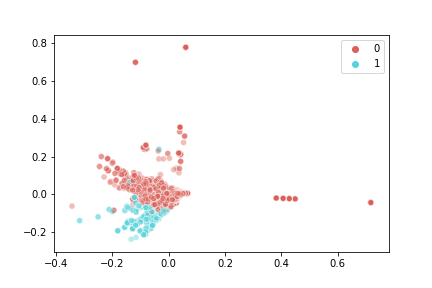
\includegraphics[width=0.45\textwidth]{images/kmeans_2d_pca_k=2.png}\label{fig:pca2k2}}
	\subfloat[3D PCA k=2]{  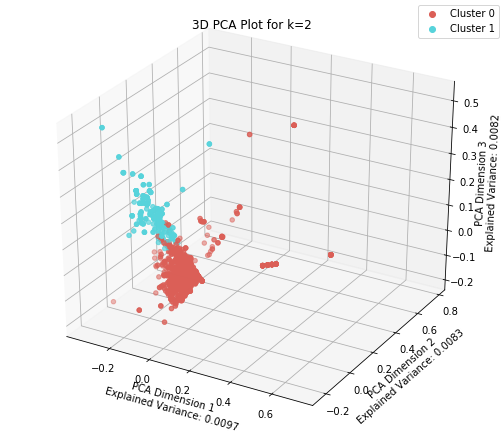
\includegraphics[width=0.45\textwidth]{images/kmeans_3d_pca_k=2.png}\label{fig:pca3k2}}\\
	\subfloat[2D T-SNE k=2]{  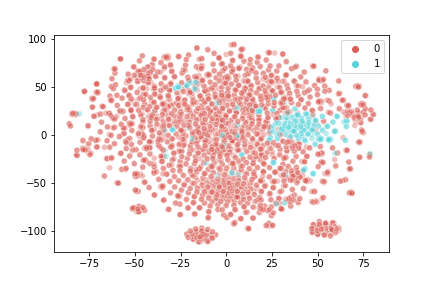
\includegraphics[width=0.45\textwidth]{images/kmeans_2d_tsne_k=2.png}\label{fig:ts2k2}}
	\subfloat[3D T-SNE k=2]{  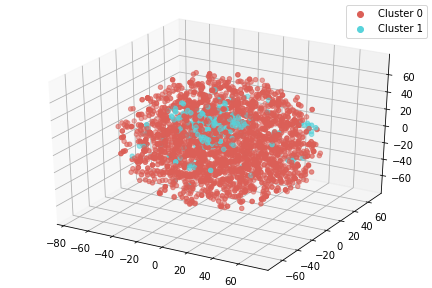
\includegraphics[width=0.45\textwidth]{images/kmeans_3d_tsne_k=2.png}\label{fig:ts3k2}}\\
	\caption{Decompositions of the clusters in 2 and 3 dimensions using PCA and T-SNE for k=2}
	\label{fig:k2pca}
\end{figure}
Examining the Mahalanobis distances for the two clusters, there does not appear to be any noticeable pattern, the distributions are slightly bimodal, compared to the Euclidean distances, which appears to be slightly normally distributed shape wise, though normality would not be expected as the 0 distance would be the cluster centre, from which the distances are measured. The majority of points are associated with cluster 0, with the rest going to Cluster 1.
\begin{figure}[H]
	\centering
	\subfloat[Mahalanobis Distance]{  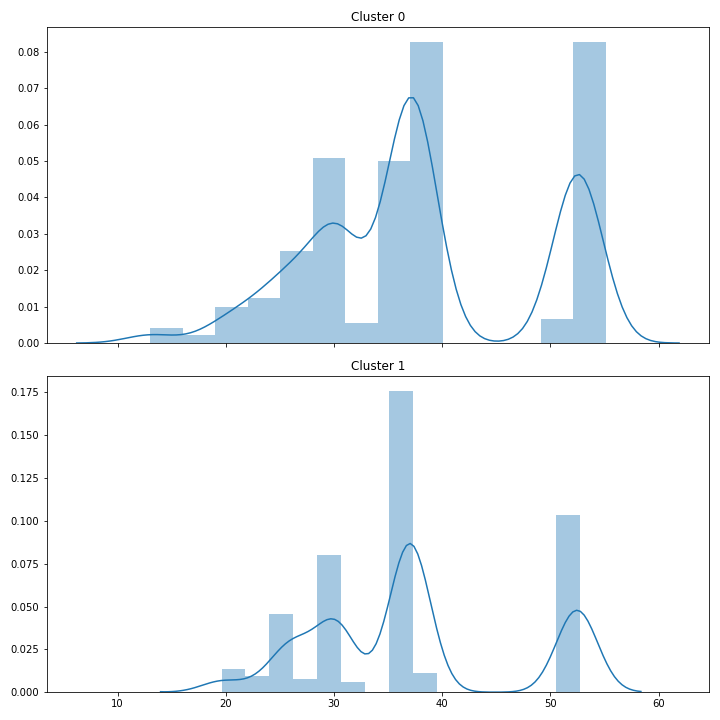
\includegraphics[width=0.45\textwidth]{images/kmeans_mahalanobis_distance_k=2.png}\label{fig:mhk2}}
	\subfloat[Euclidean Distances]{  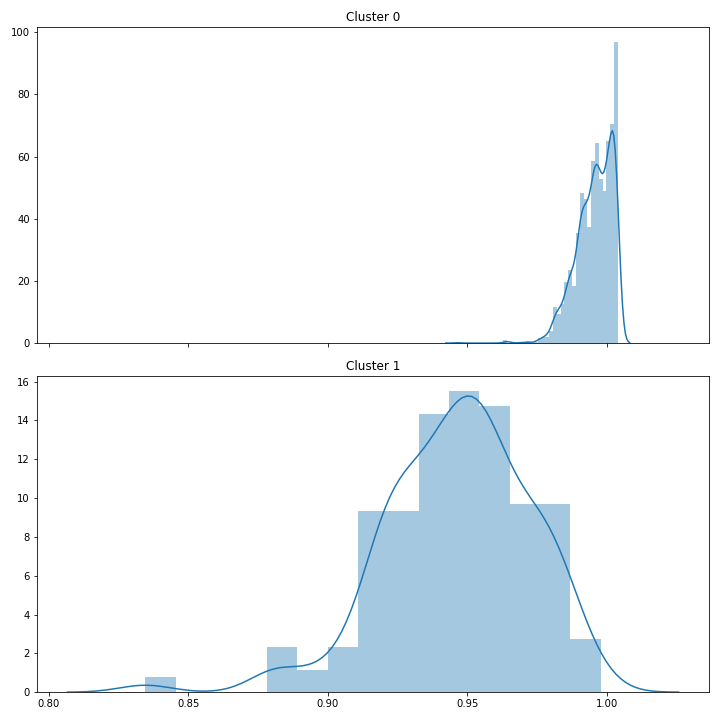
\includegraphics[width=0.45\textwidth]{images/kmeans_euclidean_distance_k=2.png}\label{fig:euk2}}\\
	
	\caption{Cluster Distances (Mahalanobis and Euclidean) for k=2 clusters}
	\label{fig:distk2}
\end{figure}

Comparing the results plotted on the log scale shown in Figure \ref{fig:wordsk2}, the first thing which becomes apparent is that the distances for the words appears to be the same between clusters, i.e. all phrases tested are equally far from both cluster 0 and cluster 1, this is perhaps unsurprising as the distance from the both clusters is extremely large. Comparing the words themselves, aside from the individual word `covid`, the phrases are fairly close together, with what appears to be two sets of lines. The first lines are the `coronavirus hits remote utah`, and the `aboriginal peoples australia complain` with the remainder of the headlines making up the remainder of the lines, nearly all of the results are between 27 and 28 in terms of the absolute logged Mahalanobis distance. 
\begin{figure}[H]
	\centering
	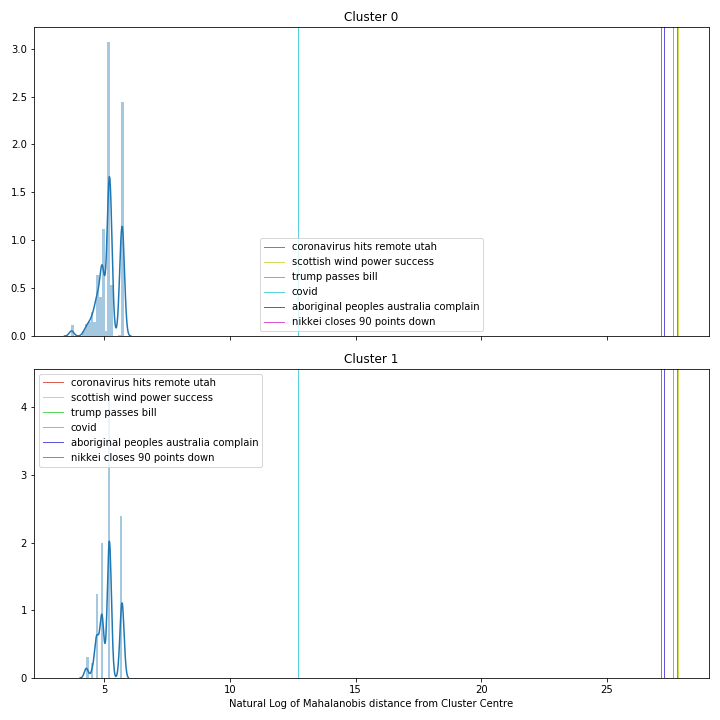
\includegraphics[width=0.8\textwidth]{images/words_kmeans_mahalanobis_distance_k=2.png}
	\caption{Log of Mahalanobis Distances for Clusters and Selected Phrases for k=2 clusters}
	\label{fig:wordsk2}
\end{figure}

\paragraph{Clustering when k=3 or k=4} 
When the number of clusters was increased to 3 or 4, it was found that there was no material change in either the topic word clouds or the decomposition plots. Thus, the word cloud, decomposition plots, and Mahalanobis distance plots are included in the appendices \ref{k3} and \ref{k4}. The word clouds for both k=3 and k=4 behaved the same as k=2, where the topics were all very similar, and the decomposition plots suggest the cluster definitions are definitively useful, and the boundaries are not as clear as they were for k=2.  There are a few features of note however. when k was 3, there were 2 sets of points away from the main cluster, but when examined, these represented the points associated with the parsing errors from the URLs. The cluster Mahalanobis distances appear to be bimodal with the same range of distances for the points. As expected, the Mahalanobis distance for the selected phrases were similar distances away, with the pattern of distances being similar.

\subsection{Modelling Stock Prices}
The table of prediction accuracies for the different models is shown in Table \ref{table:modaccuracy}. This is the percentage of days over the prediction interval of May and June that each model was able to predict correctly. Several models had similar accuracy scores, though it should be noted that the predictions were on a very small dataset, so even one or two correct incorrect predictions could sway the result considerably. 

The manually lagged models appeared to be the least best, in these models 5 days worth of previous days were added as 5 features to the data, and no other averaging methodology applied. Interestingly, the random forests classifiers appeared to do well with whatever data structure was used. Furthermore, models which applied moving window calculations did well, with on average the exponentially smoothed models doing the best.

With all of that taken into consideration, the best model was picked on the basis of being exponential and the random forests, and was found to be the exponential random forest.
\begin{table}[H]
	\centering 
\begin{tabular}{lr}

	Classifier &  Accuracy \\
	\hline
	Reference Classifier with Previous Day & 0.750\\
	\hline
                                  Naive Bayes &     0.750 \\
Logistic Regression &     0.750 \\
Averaged Random Forests &     0.750 \\
Gaussian Averaged Random Forests &     0.750 \\
Exponential Naive Bayes &     0.750 \\
Exponential Logistic Regression &     0.750 \\
Exponential Random Forests &     0.750 \\
Random Forests &     0.625 \\
Support Vector Machine &     0.625 \\
Averaged Naive Bayes &     0.625 \\
Averaged Logistic Regression &     0.625 \\
Averaged Support Vector Machine &     0.625 \\
Gaussian Averaged Naive Bayes &     0.625 \\
Gaussian Averaged Logistic Regression &     0.625 \\
Gaussian Averaged Support Vector Machine &     0.625 \\
Exponential Support Vector Machine &     0.625 \\
Manually 4 day lagged Random Forests &     0.625 \\
Neural Network & 0.500 \\
Manually 4 day lagged Naive Bayes &     0.500 \\
Manually 4 day lagged Logistic Regression &     0.500 \\
Manually 4 day lagged Support Vector Machine &     0.375 \\
	

\end{tabular}

	\caption{Table of Model Accuracy Results}
		\label{table:modaccuracy}
\end{table}

Comparing the reference model to the exponentially lagged Random Forests Model on May June Data, The reference model was 50\% accurate, and the exponentially smoothed random forest achieved an accuracy of 62.5\%, which would appear to suggest that the Average Tone and Goldstein Scale values do provide value in terms of predicting shift. 

The predictions are shown in figure \ref{fig:modelpred}, where the magnitude of the differences has been plotted, alongside whether the best model was correct in predicting a positive or negative shift (blanks are weekends or days when the stock market did not operate). There does not appear to be a time based prediction component, the model is just as likely to predict correctly or incorrectly regardless of the time that it is predicting on. Interestingly, the model does not appear to be very good at predicting for large stretches correctly, it correctly predicts for a day or two, and then has incorrect predictions for a similar length of interval. The exception to this is when halfway through the prediction, the model correctly predicts the spike and the subsequent fall and recovery. 

The distribution of magnitude of the positive and negative daily differences is plotted in Figure \ref{fig:distmodel}.  It is apparent that the model is better at predicting smaller differences in the stock market. the majority of incorrect predictions come from larger negative values closer to -500 points and slightly from the positive jumps. There are significantly fewer incorrect predictions when the market jumps between -250 and +250 points. Interestingly, there is a small bump at a large positive value of +1000, suggesting the model was good at predicting large positive values. 

\begin{figure}[H]
	\centering
	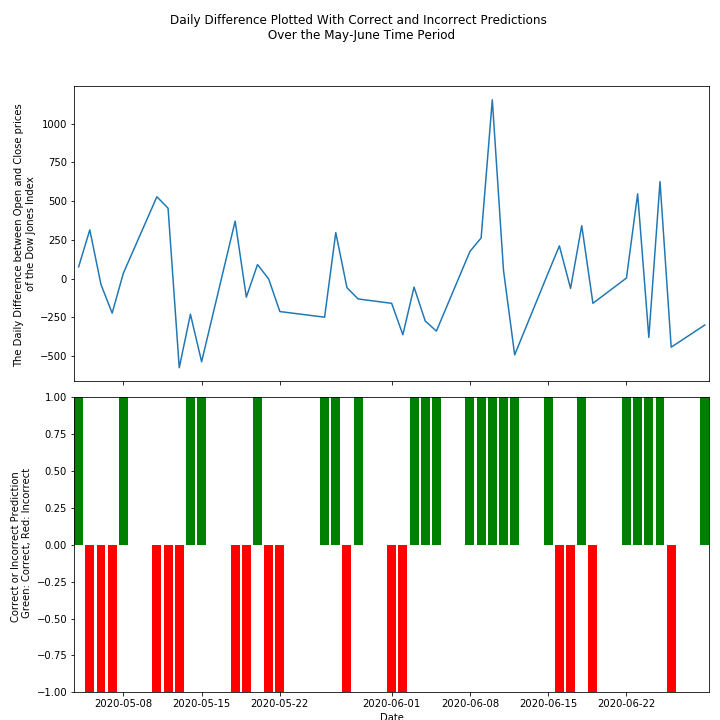
\includegraphics[width=0.8\textwidth]{images/model_pred_time.png}
	\caption{The Dow Jones daily changes in prediction dataset, and whether the model predicted the result correctly or not on a daily basis over the prediction interval of May and June 2020}
	\label{fig:modelpred}
\end{figure}


\begin{figure}[H]
	\centering
	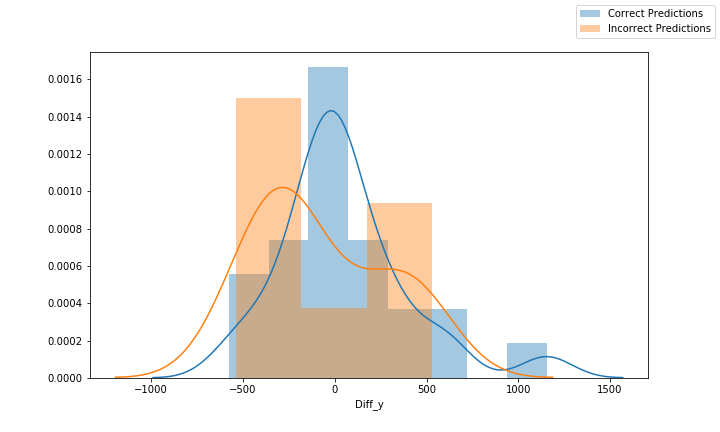
\includegraphics[width=0.8\textwidth]{images/dist_of_model.png}
	\caption{The distribution of the daily differences between open and close prices where the model predicted correctly vs predicted incorrectly}
	\label{fig:distmodel}
\end{figure}

\subsubsection{Portfolio Results}
3 different portfolio styles were tried, firstly a balanced strategy, where half of the capital is used every time shares are bought, and half of the shares are sold whenever shares are sold. This is shown in Figure \ref{fig:port_1}. The second strategy focused on maximising capital, so only \unboldmath$\frac{1}{5}$ of capital was used to buy shares, and $\frac{4}{5}$ of shares were sold whenever shares were sold. This is shown in Figure \ref{fig:port_2}. The final strategy was a shares maximising strategy where $\frac{4}{5}$ of capital was used to buy shares any time shares were brought, and $\frac{1}{5}$ of shares were sold whenever shares were sold. This is shown in Figure \ref{fig:port_3}. All of these strategies started off with no initial shares, and an initial capital of 2000, and used a prediction sensitivity threshold of 60\%. 


\begin{figure}[H]
	\centering
	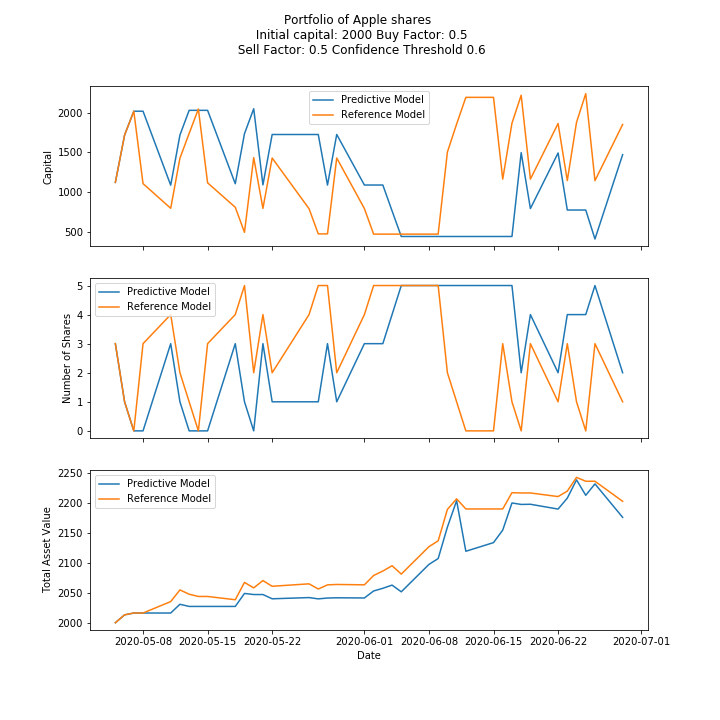
\includegraphics[width=0.65\textwidth]{images/portfolio_1.png}
	\caption{The amount of shares, capital, and Total Asset Value plotted through the time for the first portfolio strategy}
	\label{fig:port_1}
\end{figure}

\begin{figure}[H]
	\centering
	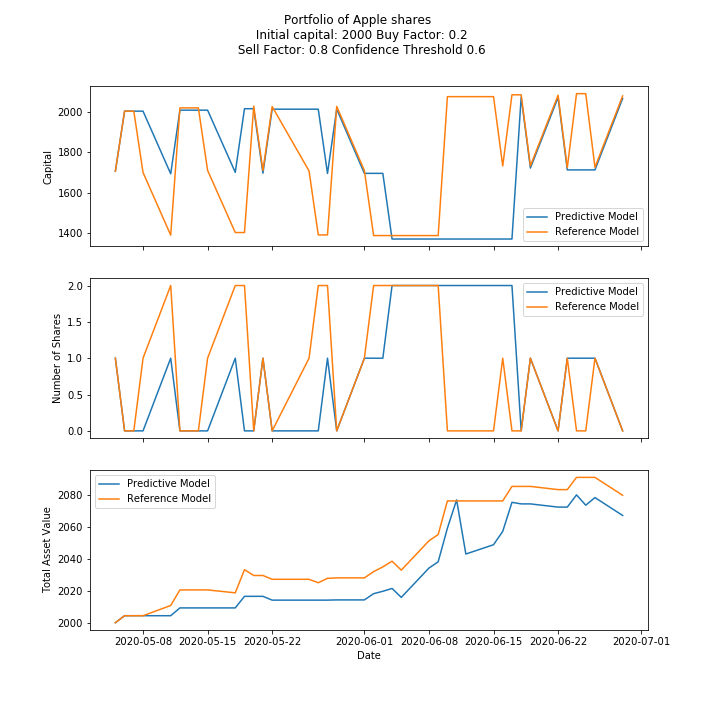
\includegraphics[width=0.65\textwidth]{images/portfolio_2.png}
	\caption{The amount of shares, capital, and Total Asset Value plotted through the time for the second portfolio strategy}
	\label{fig:port_2}
\end{figure}

\begin{figure}[H]
	\centering
	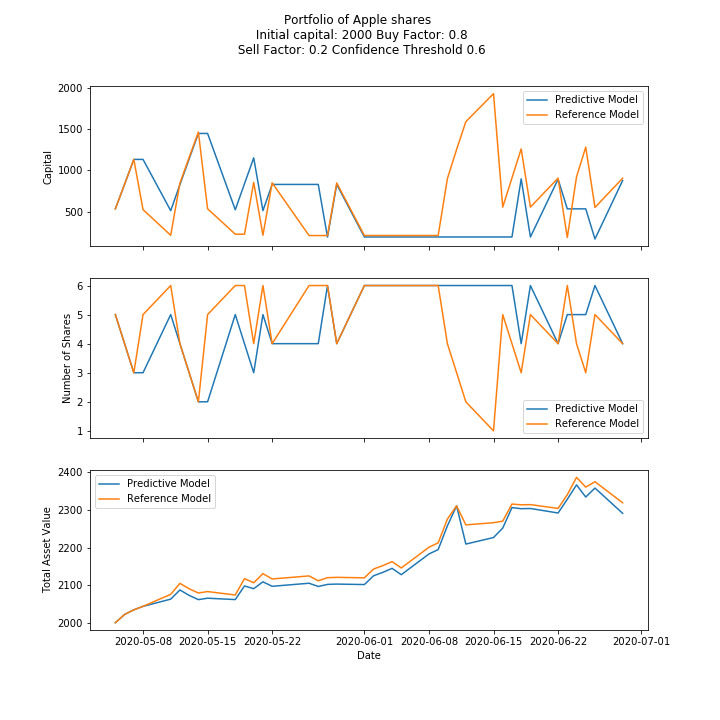
\includegraphics[width=0.65\textwidth]{images/portfolio_3.png}
	\caption{The amount of shares, capital, and Total Asset Value plotted through the time for the third portfolio strategy}
	\label{fig:port_3}
\end{figure}

The first thing to be noted in all of the strategies, is that in all cases, the predictive model was slightly worse over the time period compared to the reference model. This is mostly likely because the predictive model in all cases held on to the stock around the 10th of June, after which the value of the stock decreased considerably and the model was not able to make up the difference within the remaining time period. The second point to be made is that all of the strategies accrued financial gain, though the model to maximise shares had the highest total asset value at the end of the time period, followed by the half and half strategy, followed by the capital strategy. The shares total asset value at the end was significantly beyond 2200, which represents more than a 10\% gain in the market over the initial capital investment. However, by comparison the maximising capital strategy only achieved an asset value of 2060, which is a significantly lower growth. The half capital and half shares strategy was doing well, especially recovering after the drop in the middle of the month, but it fell slightly to record a value of nearly 2200, which still is nearly a 10\% gain. 


\section{Discussion}
\label{discussion}
The broader purpose of topic modelling was to build a topic model which would be able to categorise new and upcoming geopolitical risks, and thus be able to filter through only the relevant information. In the context of using GDELT, it would mean filtering out the headlines to only use the tone and Goldstein scale values of events where the headlines were related to the topic doing the filtering. This would mean that the topic model would not only have to be able to curate existing risks adequately, but also be able to catch new emerging risks too.

After performing the cluster analysis, and topic modelling, there were several things which became apparent. Firstly, the topic models are good at finding the main topics. Both the clusters and the LDA topic models were able to find what would be considered the `main` words in the topic, in that if a human were to look for the most important words, this is what they would be. Furthermore, if the TF-IDF results were examined, the results were surprisingly insightful into the data. The results were mostly coherent and representative of what a human would achieve for the time period of the training data.

However, one of the main concerns for both the LDA model and the clustering algorithm is the lack of separability. In both of the topic modelling attempts it appeared that there was only ever one topic being detected, in that there was no separation between the words such as `china` and `coronavirus`. This could perhaps be a result of there not being at least two topics present in the data. However, comparing the single day data and the USA China data, neither set of word clouds strongly show a prevailing topic, though both represent the data reasonably. This in itself is extremely promising, as the corpus and documents themselves were composed of URLs which were brute force parsed, which in turn meant that there was a lot of `garbage` data in the corpus, the result of parsed URLs where the headline was not coherent or even not there.

The main concern with the topic models is the fact that existing topic models cannot be used effectively in terms of filtering words, phrases, or topics unknown to the historical topic development, and thus cannot detect new topics. One of the biggest issues with LDA models is that the documents themselves have been generated from a specific set of topics, which means that if the word being filtered did not exist in the corpus there is no probability/closeness metric that can generated for each topic. This means that one of the only ways a topic model could be used for new data is if a dictionary was used to generate the corpus along with the news media at hand. This in turn would create two other problems. Firstly, it would disrupt the meaning of the topics as there would be an excess of unrelated words to the documents, this however could theoretically be solved by using extremely large datasets, and significantly larger amounts of processing power. The second issue with this approach is more prohibitive. New words and topics appear constantly in the media. For example, a topic model in November would not have been able to predict the importance of topics associated with Coronavirus. This is especially problematic for geopolitical modelling, as often it would be events appearing out of the blue which cause the most amount of disruption. This problem is not fixable by any amount of data or processing power, as no dataset can ever be complete indefinitely, new words/topics will always appear in the data.  

A similar problem exists for K-Means. The K-Means algorithm for words in this instance uses the TF-IDF vectorization to build clusters. This relies upon all of the words existing in corpus in a manner where the most common important words appear most frequently. This means inherently the weighting is designed for a fully complete corpus, and not one which is being used to analyse new information. One of the main differences between the K-Means algorithm and the LDA algorithm is that for K-Means it is possible to get a quantitative distance measure for a word not originally in the corpus to a particular cluster centre, as TF-IDF weightings can be calculated by inserting an offset for words which are not in the corpus. However, this means that the distances to the cluster centres for words not in the corpus are much less useful. There is no way for an existing cluster model to tell apart a new rising topic from information which is irrelevant or noise as both would have the same calculated TF-IDF value with regards to the corpus the TF-IDF is calculated from. For example a pre-covid trained cluster model, words related to coronavirus or covid would be categorised as noise or irrelevant instead of an upcoming rising topic.

This is shown in Figures \ref{fig:wordsk2}, \ref{fig:wordsk3}, and \ref{fig:wordsk4}. The results were plotted on a log scale, as distances between points for words and clusters can be significantly larger than the distances within clusters. Firstly, it becomes apparent that it does not matter which cluster is chosen in terms of calculating Mahalanobis distance for a new word or phrase, because all of the clusters are so close together, and the vectorised words are so far away. This means that when the log of the distance is taken, plotting the results mean that for each of the clusters the distance is exactly the same. 

Furthermore, some phrases do appear closer to any and all of the clusters than other phrases. This seems promising, as specifically the `coronavirus hits remote utah` is a relevant headline to the topic being detected, and thus it being closer suggests it might be useful. However, the difference on the log scale between that phrase and a totally irrelevant phrase (aboriginal peoples australia complain) is barely noticeable which furthers the idea that the TF-IDF is transforming relevant and `garbage` information in the same way. The single word `covid` is considerably closer, but a headline would rarely consist of only a single word, and more pertinently, in terms of relative distance for points within the cluster it is still orders of magnitude away. These plots also show that the low explained variance in the PCA decomposed dimensions isn't just a problem with the dimension picked, but rather is indicative of the clusters not being able to cluster the data effectively. 

As such this was the main reason the topic model was not used for filtering for a secondary dataset and why this approach in this fashion appears to not be useful in fashion for the task being attempted. Moreover, one of the biggest challenges with this work is that the topic models only work on a single word basis. All of the clusters and LDA models are based on single words, and not phrases, or content. This means there would still have to be a large amount of manual work required when using this approach, to ensure that the algorithms do not end up working with incoherence. The principle of garbage in garbage out also applies here, there is a substantial amount of preprocessing required to ensure that you're feeding the algorithm useful information, and even after that it is not guaranteed if the content is capable of making clusters or not.

Looking at the results from the stock prediction models, it is difficult to say with any certainty what the best model is. The models were only trained on 2 months worth of data, which is not sufficient to conclusively identify which model is the `best`, or at least most accurate. However, there are certain features of the models which become apparent, generally weighted models deal well with the data, the manually lagged non-weighted model was certainly the worst off of all of the models which were tried. This does back up the theory that the Average Tone and the Goldstein Score may influence stock prices several days down the line, with the most important day being the last day in the moving window. 

Looking at the model structures, the Random Forests classifiers did well with whatever style of smoothing performed on the data, suggesting that a Tree based approach may provide better results for this sort of problem. Examining the results of the `best` random forests model, it appears the model finds success in predicting upwards, and predicting small changes in the market. However, the model struggles with predicting shock falls in the stock market, which most likely would not be captured in any information available to the model.  

This shock also explains the difference in portfolios between the best Random Forests model and the reference model. The best Random Forests model around the middle of June completely missed the crash in the market, and held onto the stock which meant that in all of the strategies tried, the model wouldn't after that be able to catch up to the `reference` model. Interestingly, the reference model \textit{was} able to capture the fall in the middle of June, as in all three strategies, the model sold the stock, and thus didn't suffer a fall in total asset value. This reference model was only based on the previous day's prices, whereas the `best` model used the Average Tone and Goldstein Scale values as well. However, the previous day's feature importance was much less for the best model, shown in Figure \ref{fig:featimport}, so any internal pattern that the previous day was able to show to predict the fall, if present, may have been ignored as that feature was less useful. 

One of the other issues with this prediction interval is that the data restricts what the model has learned on. The stock market went through remarkable changes over this period, and for large periods of time, there is no guarantee that this would be representative of regular behaviour on the stock market. Longer term more stable predictions would be more useful for investors looking to invest over the long term, as this strategy will over a longer period of time generally offer better results than short term investing.

It should also be noted that any analysis of potential monetary gain which might arise from using a model would have to be compared against stock market long term growth, as for the model to be fully useful, it would mean that it would be able to make gains \textit{beyond} the normal growth of the market. This was shown in the stock maximising strategy, where the total asset value was greater than the 9.5\% annual growth. 






\section{Conclusions}
\label{conclusions}
The aim of this dissertation was to use the GDELT database to build topic models from news headlines, and if that were successful to use the topic model as a filter to collect relevant news which contained topics similar to the topic model, and then use the Conflict Cooperation Goldstein scale as a geopolitical risk measure to predict against the stock market. 

There were several approaches to calculating geopolitical risk in the past which work from manually calculating occurrences of key words in news articles. This dissertation used a pre-existing Conflict Cooperation scale from events as a measure of geopolitical risk, with the main filtering occurring by choosing which events to factor in based on the headlines of those events.  The original attempt for topic modelling was to use a LDA model on restricted data to attempt to separate topics.    

It was found that despite changing the number of topics being used it was unable to provide a quantitative value for unseen information, as all information which could be classified would have to exist in the corpus when the topic model was created, which would mean that it cannot detect new topics occurring. This meant that this approach would not be usable, as it would not be able to detect new topics.

Thus to try to gain a more quantitative approach, the K-means algorithm was used alongside TF-IDF vectorization, which would  firstly build clusters of words in an attempt to collate the individual topics present into those clusters. Then the aim was to use the Mahalanobis distance between cluster centres and unseen headlines and news to filter out or weight headlines which are relevant to the topic or not by how close they are to the cluster. The Mahalanobis distance was used as it provides a standardised measurement of the distance between, which isn't going to be affected by the shape of the cluster. 

However, the main issue which occurred with this approach is that there was no useful cluster separation occurring. The cluster definitions were all not as expected in terms of clustering. However the main issue with this was that the distance metric for unseen headlines and news was not useful. The TF-IDF metric meant that the algorithm placed new information the same as noise and irrelevant data. Thus this too would not be able to be used as it would not be able to distinguish new topics, nor was it able to provide distance calculations accurately for filtering purposes.

Since neither of the topic modelling approaches appeared to work effectively, the modelling was done on the GDELT data filtered via Google Big Query in GDELT itself, as opposed to filtered through the topic models. The models used were classification models which aimed to predict stock shift up or down. These models appeared to be reasonably accurate, with the best of them being more accurate on a separate set of data as compared to a reference model which just used the previous day's data. Only a few model types and strategies were explored in this dissertation, there is definitely the potential in terms of further work to explore other different types of models.

Over the course of this dissertation, several topic modelling algorithms were built, but they ran into the problem of the topics and clusters being too close together, and thus neither the topics nor the clusters were distinct. More pertinently the issue of cluster and topic models being designed to work on a complete dataset, and not providing accurate results for unseen data was the main reason why this approach was thought to not work in this fashion. These algorithms might work if the data was more carefully selected with regards to Tf-IDF values, but it does not appear to be useful in this manner. With regards to the models, there always remains more scope for trying different types of models which may present more accurate results, but the preliminary results appear to suggest that the Goldstein score and the Average tone might both be useful in terms of predicting on the stock market.


\section{Further Work}
This dissertation was an attempt into seeing if the Goldstein scale alongside the Average Tone from the GDELT database can be used as a measure of geopolitical risk and calculated against the curated parts of the Stock Market. There is a large amount of further work which can be explored from this, in all aspects, from the topic modelling, to the modelling of Average Tone against the Goldstein Scale. 

One of the most apparent extensions of this work would be to try these methods on more data. GDELT is a large resource, and a vast amount of data is available to be explored and tried, from data from multiple other countries, to using more historical long term data. 

Furthermore, from these experiments alone it appears unlikely that topic modelling can be used in the way that it was initially thought in this dissertation. Even if the distance metrics are relatively accurate for new words and phrases, the topic models by design will inherently not be able to detect the presence of new topics, which would be a key aspect of this.

Another extension which could be performed is to use a method which works on more than just one word at a time. Both the TF-IDF K-Means and LDA model approaches work on a single word basis, which may not be enough to sufficiently separate the topics, thus an approach which takes into consideration phrases or bigrams may allow for more context to be explored which in turn may lead to better separability within the topics. 

One of the other main features which could be explored from a more modelling perspective could be an attempt to predict the stock shift in a more fine grained manner, this work only aimed to predict any changes in stock, and as a result this does not take magnitude of change into consideration, a large stock fall is the same as a small stock fall, but investor reactions may be different if it is only a minor fall in the market, thus being able to predict small, medium, or large shifts may become useful in the long term. 

Another factor which was not modelled was building autoregressive style lagging for the stock prices themselves, along with the lagged models for the Average Tone and the Goldstein Scale. 


\appendix



\begin{appendices}
	\section{Phrases to Test K-Means}
	The phrases with which the K-Means algorithm was tested are shown below:
	\label{phrases}
\renewcommand\labelitemi{---}
	\begin{itemize}
\item 			 coronavirus hits remote utah
		\item scottish wind power success 
\item 		trump passes bill
		\item covid
		\item aboriginal peoples australia complain
		\item nikkei closes 90 points down
	\end{itemize}

	\section{K-Means Clustering k=3}
	\label{k3}
	\begin{figure}[H]
		\centering
		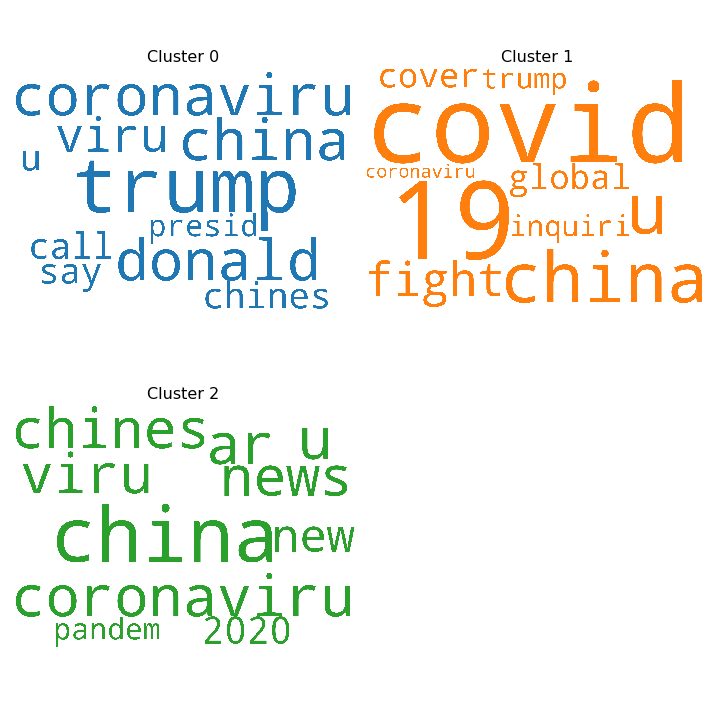
\includegraphics[width=0.8\textwidth]{images/kmeans_word_cloud_k=3.png}
		\caption{Word Cloud for k=3 clusters}
		\label{fig:wck3}
	\end{figure}
	
	\begin{figure}[H]
		\centering
		\subfloat[2D PCA k=3]{  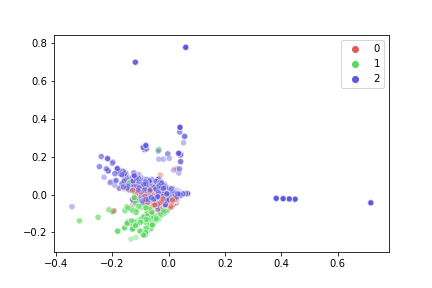
\includegraphics[width=0.45\textwidth]{images/kmeans_2d_pca_k=3.png}\label{fig:pca2k3}}
		\subfloat[3D PCA k=3]{  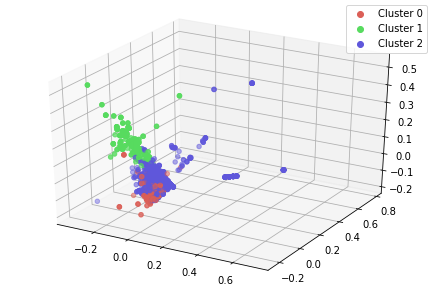
\includegraphics[width=0.45\textwidth]{images/kmeans_3d_pca_k=3.png}\label{fig:pca3k3}}\\
		\subfloat[2D T-SNE k=3]{  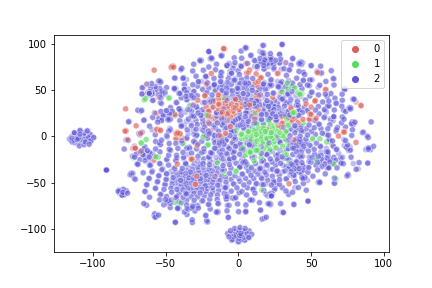
\includegraphics[width=0.45\textwidth]{images/kmeans_2d_tsne_k=3.png}\label{fig:ts2k3}}
		\subfloat[3D T-SNE k=3]{  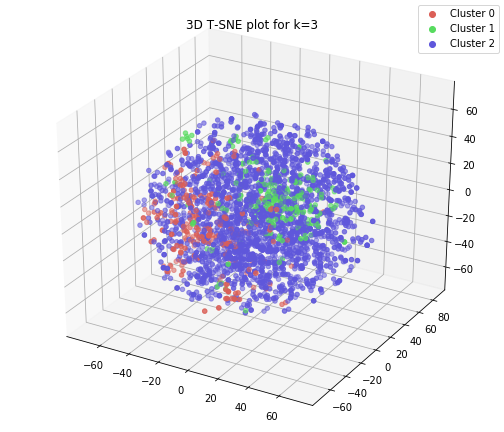
\includegraphics[width=0.45\textwidth]{images/kmeans_3d_tsne_k=3.png}\label{fig:ts3k3}}\\
		\caption{Decompositions of the clusters in 2 and 3 dimensions using PCA and T-SNE for k=3}
		\label{fig:k3pca}
	\end{figure}
	
	\begin{figure}[H]
		\centering
		\subfloat[Mahalanobis Distance]{  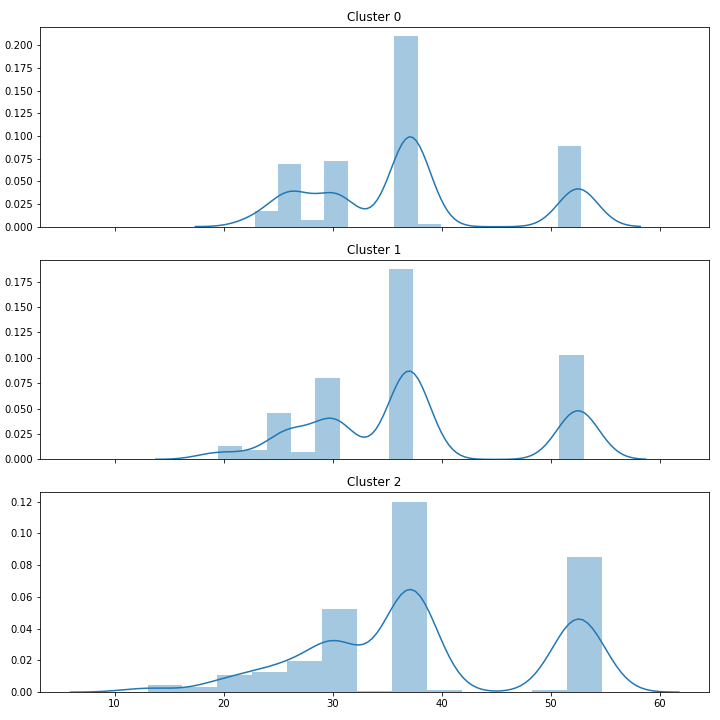
\includegraphics[width=0.45\textwidth]{images/kmeans_mahalanobis_distance_k=3.png}\label{fig:mhk3}}
		\subfloat[Euclidean Distances]{  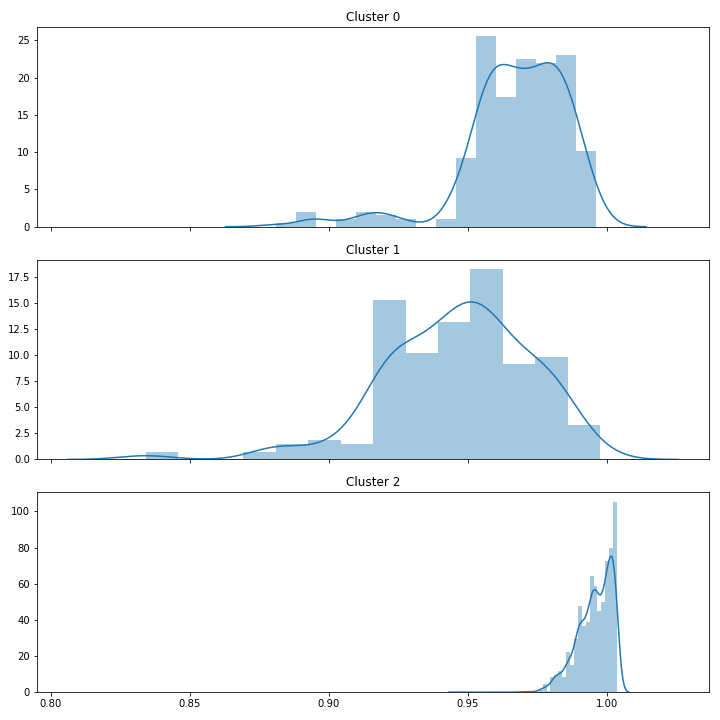
\includegraphics[width=0.45\textwidth]{images/kmeans_euclidean_distance_k=3.png}\label{fig:euk3}}\\
		
		\caption{Cluster Distances (Mahalanobis and Euclidean) for k=3 clusters}
		\label{fig:distk3}
	\end{figure}
	
	\begin{figure}[H]
		\centering
		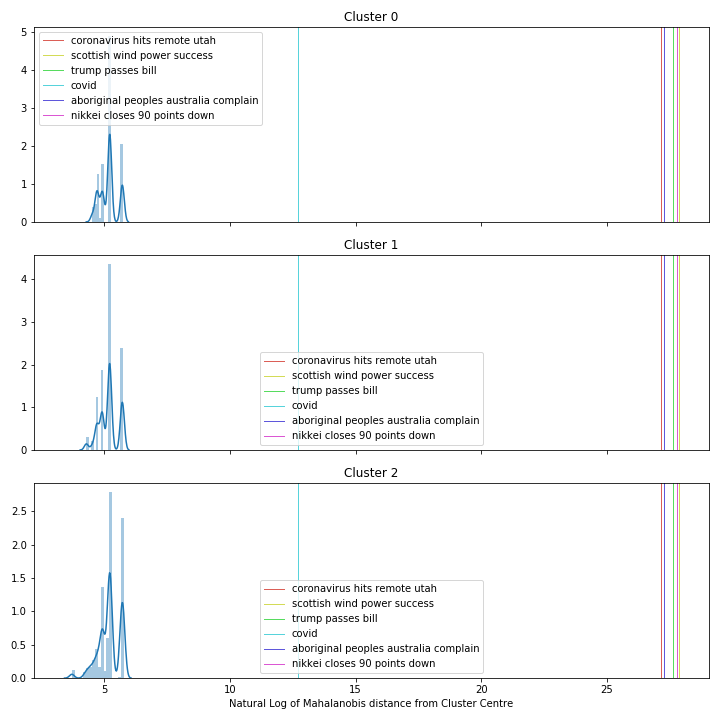
\includegraphics[width=0.8\textwidth]{images/words_kmeans_mahalanobis_distance_k=3.png}
		\caption{Log of Mahalanobis Distances for Clusters and Selected Phrases for k=3 clusters}
		\label{fig:wordsk3}
	\end{figure}
	\section{K-Means Clustering k=4}
	\label{k4}
	\begin{figure}[H]
		\centering
		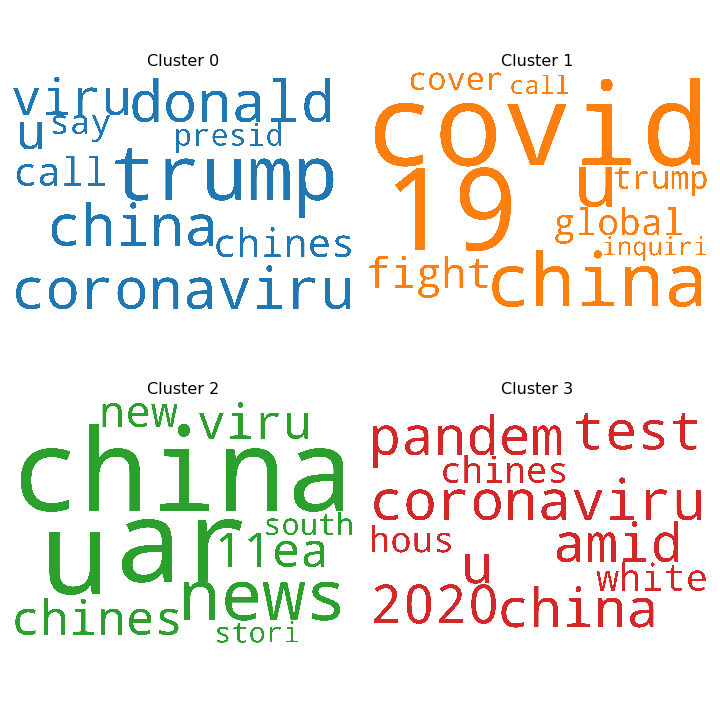
\includegraphics[width=0.8\textwidth]{images/kmeans_word_cloud_k=4.png}
		\caption{Word Cloud for k=4 clusters}
		\label{fig:wck4}
	\end{figure}
	
	
	\begin{figure}[H]
		\centering
		\subfloat[2D PCA k=4]{  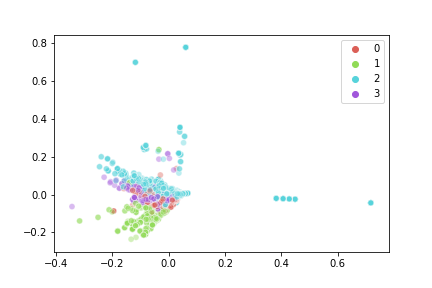
\includegraphics[width=0.45\textwidth]{images/kmeans_2d_pca_k=4.png}\label{fig:pca2k4}}
		\subfloat[3D PCA k=4]{  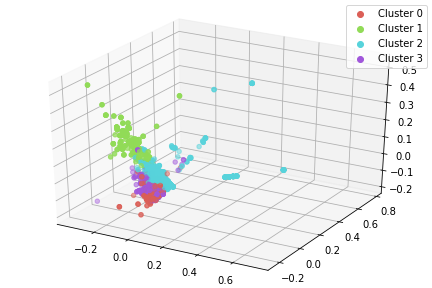
\includegraphics[width=0.45\textwidth]{images/kmeans_3d_pca_k=4.png}\label{fig:pca3k4}}\\
		\subfloat[2D T-SNE k=4]{  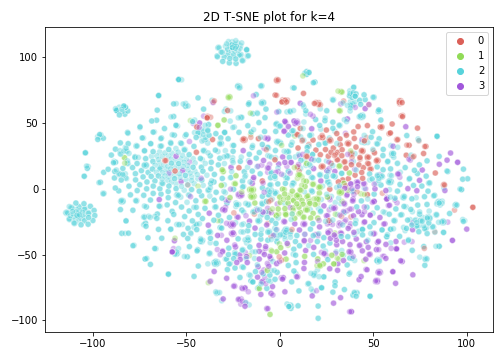
\includegraphics[width=0.45\textwidth]{images/kmeans_2d_tsne_k=4.png}\label{fig:ts2k4}}
		\subfloat[3D T-SNE k=4]{  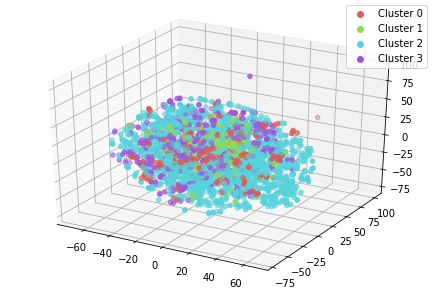
\includegraphics[width=0.45\textwidth]{images/kmeans_3d_tsne_k=4.png}\label{fig:ts3k4}}\\
		\caption{Decompositions of the clusters in 2 and 3 dimensions using PCA and T-SNE for k=4}
		\label{fig:k4pca}
	\end{figure}
	
	\begin{figure}[H]
		\centering
		\subfloat[Mahalanobis Distance]{  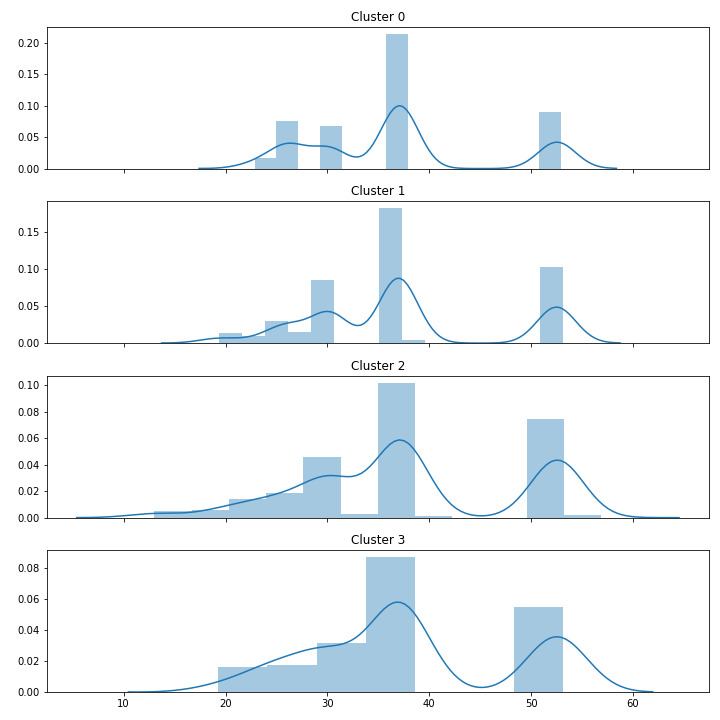
\includegraphics[width=0.45\textwidth]{images/kmeans_mahalanobis_distance_k=4.png}\label{fig:mhk4}}
		\subfloat[Euclidean Distances]{  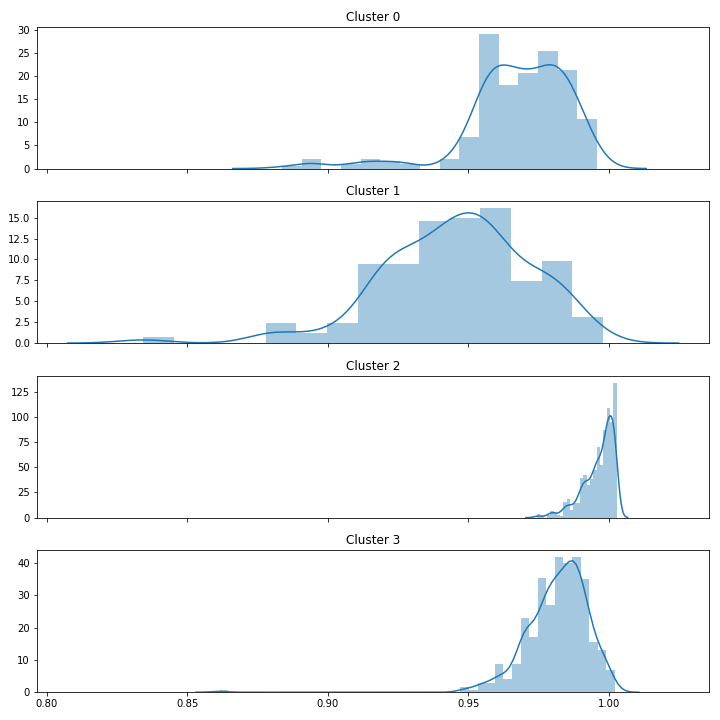
\includegraphics[width=0.45\textwidth]{images/kmeans_euclidean_distance_k=4.png}\label{fig:euk4}}\\
		
		\caption{Cluster Distances (Mahalanobis and Euclidean) for k=4 clusters}
		\label{fig:distk4}
	\end{figure}
	
	
	\begin{figure}[H]
		\centering
		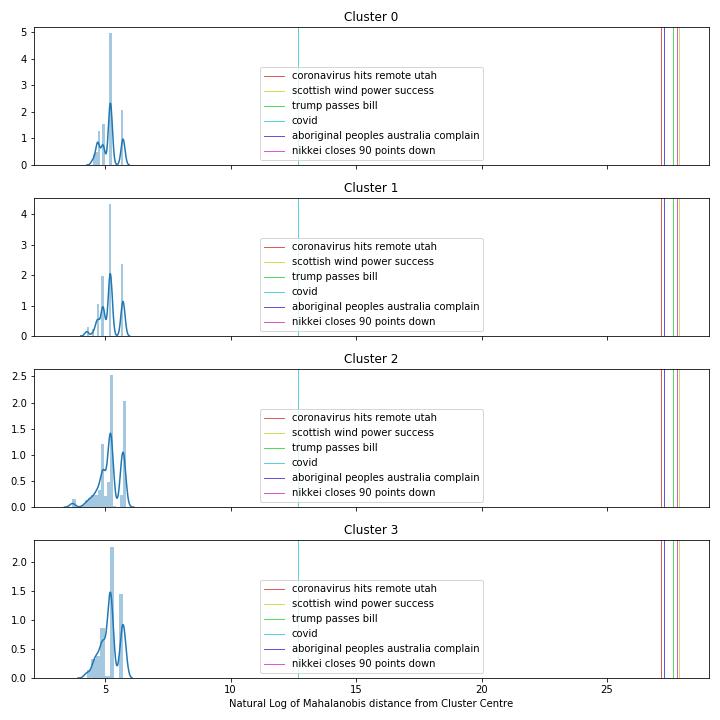
\includegraphics[width=0.8\textwidth]{images/words_kmeans_mahalanobis_distance_k=4.png}
		\caption{Log of Mahalanobis Distances for Clusters and Selected Phrases for k=4 clusters}
		\label{fig:wordsk4}
	\end{figure}
\end{appendices}


\bibliographystyle{acm}
\bibliography{ref}
\end{document}
